\documentclass[a4paper]{article}

\def\npart {III}
\def\nterm {Michaelmas}
\def\nyear {2016}
\def\nlecturer {B. Allanach}
\def\ncourse {Quantum Field Theory}
\def\nlectures {TTS.12}

% Imports
\ifx \nextra \undefined
  \usepackage[pdftex,
    hidelinks,
    pdfauthor={Dexter Chua},
    pdfsubject={Cambridge Maths Notes: Part \npart\ - \ncourse},
    pdftitle={Part \npart\ - \ncourse},
  pdfkeywords={Cambridge Mathematics Maths Math \npart\ \nterm\ \nyear\ \ncourse}]{hyperref}
  \title{Part \npart\ - \ncourse}
\else
  \usepackage[pdftex,
    hidelinks,
    pdfauthor={Dexter Chua},
    pdfsubject={Cambridge Maths Notes: Part \npart\ - \ncourse\ (\nextra)},
    pdftitle={Part \npart\ - \ncourse\ (\nextra)},
  pdfkeywords={Cambridge Mathematics Maths Math \npart\ \nterm\ \nyear\ \ncourse\ \nextra}]{hyperref}

  \title{Part \npart\ - \ncourse \\ {\Large \nextra}}
\fi

\author{Lectured by \nlecturer \\\small Notes taken by Dexter Chua}
\date{\nterm\ \nyear}

\usepackage{alltt}
\usepackage{amsfonts}
\usepackage{amsmath}
\usepackage{amssymb}
\usepackage{amsthm}
\usepackage{booktabs}
\usepackage{caption}
\usepackage{enumitem}
\usepackage{fancyhdr}
\usepackage{graphicx}
\usepackage{mathtools}
\usepackage{microtype}
\usepackage{multirow}
\usepackage{pdflscape}
\usepackage{pgfplots}
\usepackage{siunitx}
\usepackage{tabularx}
\usepackage{tikz}
\usepackage{tkz-euclide}
\usepackage[normalem]{ulem}
\usepackage[all]{xy}

\pgfplotsset{compat=1.12}

\pagestyle{fancyplain}
\lhead{\emph{\nouppercase{\leftmark}}}
\ifx \nextra \undefined
  \rhead{
    \ifnum\thepage=1
    \else
      \npart\ \ncourse
    \fi}
\else
  \rhead{
    \ifnum\thepage=1
    \else
      \npart\ \ncourse\ (\nextra)
    \fi}
\fi
\usetikzlibrary{arrows}
\usetikzlibrary{decorations.markings}
\usetikzlibrary{decorations.pathmorphing}
\usetikzlibrary{positioning}
\usetikzlibrary{fadings}
\usetikzlibrary{intersections}
\usetikzlibrary{cd}

\newcommand*{\Cdot}{\raisebox{-0.25ex}{\scalebox{1.5}{$\cdot$}}}
\newcommand {\pd}[2][ ]{
  \ifx #1 { }
    \frac{\partial}{\partial #2}
  \else
    \frac{\partial^{#1}}{\partial #2^{#1}}
  \fi
}

% Theorems
\theoremstyle{definition}
\newtheorem*{aim}{Aim}
\newtheorem*{axiom}{Axiom}
\newtheorem*{claim}{Claim}
\newtheorem*{cor}{Corollary}
\newtheorem*{defi}{Definition}
\newtheorem*{eg}{Example}
\newtheorem*{fact}{Fact}
\newtheorem*{law}{Law}
\newtheorem*{lemma}{Lemma}
\newtheorem*{notation}{Notation}
\newtheorem*{prop}{Proposition}
\newtheorem*{thm}{Theorem}

\renewcommand{\labelitemi}{--}
\renewcommand{\labelitemii}{$\circ$}
\renewcommand{\labelenumi}{(\roman{*})}

\let\stdsection\section
\renewcommand\section{\newpage\stdsection}

% Strike through
\def\st{\bgroup \ULdepth=-.55ex \ULset}

% Maths symbols
\newcommand{\bra}{\langle}
\newcommand{\ket}{\rangle}

\newcommand{\N}{\mathbb{N}}
\newcommand{\Z}{\mathbb{Z}}
\newcommand{\Q}{\mathbb{Q}}
\renewcommand{\H}{\mathbb{H}}
\newcommand{\R}{\mathbb{R}}
\newcommand{\C}{\mathbb{C}}
\newcommand{\Prob}{\mathbb{P}}
\renewcommand{\P}{\mathbb{P}}
\newcommand{\E}{\mathbb{E}}
\newcommand{\F}{\mathbb{F}}
\newcommand{\cU}{\mathcal{U}}
\newcommand{\RP}{\mathbb{RP}}
\newcommand{\CP}{\mathbb{CP}}

\newcommand{\ph}{\,\cdot\,}

\DeclareMathOperator{\sech}{sech}
\DeclareMathOperator{\cosech}{cosech}
\DeclareMathOperator{\cosec}{cosec}

\DeclareMathOperator{\covol}{covol}
\DeclareMathOperator{\vol}{vol}

\let\Im\relax
\let\Re\relax
\DeclareMathOperator{\Im}{Im}
\DeclareMathOperator{\Re}{Re}
\DeclareMathOperator{\im}{im}
\DeclareMathOperator{\image}{image}
\DeclareMathOperator{\Ann}{Ann}

\DeclareMathOperator*{\res}{res}
\DeclareMathOperator{\Res}{Res}
\DeclareMathOperator{\Ind}{Ind}

\DeclareMathOperator{\tr}{tr}
\DeclareMathOperator{\diag}{diag}
\DeclareMathOperator{\rank}{rank}
\DeclareMathOperator{\card}{card}
\DeclareMathOperator{\spn}{span}
\DeclareMathOperator{\adj}{adj}

\DeclareMathOperator{\erf}{erf}
\DeclareMathOperator{\erfc}{erfc}

\DeclareMathOperator{\ord}{ord}
\DeclareMathOperator{\Sym}{Sym}

\DeclareMathOperator{\sgn}{sgn}
\DeclareMathOperator{\orb}{orb}
\DeclareMathOperator{\stab}{stab}
\DeclareMathOperator{\ccl}{ccl}

\DeclareMathOperator{\lcm}{lcm}
\DeclareMathOperator{\hcf}{hcf}

\DeclareMathOperator{\Int}{Int}
\DeclareMathOperator{\id}{id}

\DeclareMathOperator{\betaD}{beta}
\DeclareMathOperator{\gammaD}{gamma}
\DeclareMathOperator{\Poisson}{Poisson}
\DeclareMathOperator{\binomial}{binomial}
\DeclareMathOperator{\multinomial}{multinomial}
\DeclareMathOperator{\Bernoulli}{Bernoulli}
\DeclareMathOperator{\like}{like}

\DeclareMathOperator{\var}{var}
\DeclareMathOperator{\cov}{cov}
\DeclareMathOperator{\bias}{bias}
\DeclareMathOperator{\mse}{mse}
\DeclareMathOperator{\corr}{corr}

\DeclareMathOperator{\otp}{otp}
\DeclareMathOperator{\dom}{dom}

\DeclareMathOperator{\Root}{Root}
\DeclareMathOperator{\supp}{supp}
\DeclareMathOperator{\rel}{rel}
\DeclareMathOperator{\Hom}{Hom}
\DeclareMathOperator{\Aut}{Aut}
\DeclareMathOperator{\Gal}{Gal}
\DeclareMathOperator{\Mat}{Mat}
\DeclareMathOperator{\End}{End}
\DeclareMathOperator{\Char}{char}
\DeclareMathOperator{\ev}{ev}
\DeclareMathOperator{\St}{St}
\DeclareMathOperator{\Lk}{Lk}
\DeclareMathOperator{\disc}{disc}
\DeclareMathOperator{\Isom}{Isom}
\DeclareMathOperator{\length}{length}
\DeclareMathOperator{\energy}{energy}
\DeclareMathOperator{\area}{area}
\DeclareMathOperator{\Syl}{Syl}
\DeclareMathOperator{\cl}{cl}
\DeclareMathOperator{\fix}{fix}

\newcommand{\GL}{\mathrm{GL}}
\newcommand{\SL}{\mathrm{SL}}
\newcommand{\PGL}{\mathrm{PGL}}
\newcommand{\PSL}{\mathrm{PSL}}
\newcommand{\PSU}{\mathrm{PSU}}
\newcommand{\Or}{\mathrm{O}}
\newcommand{\SO}{\mathrm{SO}}
\newcommand{\U}{\mathrm{U}}
\newcommand{\SU}{\mathrm{SU}}

\renewcommand{\d}{\mathrm{d}}
\newcommand{\D}{\mathrm{D}}

\tikzset{->/.style = {decoration={markings,
                                  mark=at position 1 with {\arrow[scale=2]{latex'}}},
                      postaction={decorate}}}
\tikzset{<-/.style = {decoration={markings,
                                  mark=at position 0 with {\arrowreversed[scale=2]{latex'}}},
                      postaction={decorate}}}
\tikzset{<->/.style = {decoration={markings,
                                   mark=at position 0 with {\arrowreversed[scale=2]{latex'}},
                                   mark=at position 1 with {\arrow[scale=2]{latex'}}},
                       postaction={decorate}}}
\tikzset{->-/.style = {decoration={markings,
                                   mark=at position #1 with {\arrow[scale=2]{latex'}}},
                       postaction={decorate}}}
\tikzset{-<-/.style = {decoration={markings,
                                   mark=at position #1 with {\arrowreversed[scale=2]{latex'}}},
                       postaction={decorate}}}

\tikzset{circ/.style = {fill, circle, inner sep = 0, minimum size = 3}}
\tikzset{mstate/.style={circle, draw, blue, text=black, minimum width=0.7cm}}

\definecolor{mblue}{rgb}{0.2, 0.3, 0.8}
\definecolor{morange}{rgb}{1, 0.5, 0}
\definecolor{mgreen}{rgb}{0.1, 0.4, 0.2}
\definecolor{mred}{rgb}{0.5, 0, 0}

\def\drawcirculararc(#1,#2)(#3,#4)(#5,#6){%
    \pgfmathsetmacro\cA{(#1*#1+#2*#2-#3*#3-#4*#4)/2}%
    \pgfmathsetmacro\cB{(#1*#1+#2*#2-#5*#5-#6*#6)/2}%
    \pgfmathsetmacro\cy{(\cB*(#1-#3)-\cA*(#1-#5))/%
                        ((#2-#6)*(#1-#3)-(#2-#4)*(#1-#5))}%
    \pgfmathsetmacro\cx{(\cA-\cy*(#2-#4))/(#1-#3)}%
    \pgfmathsetmacro\cr{sqrt((#1-\cx)*(#1-\cx)+(#2-\cy)*(#2-\cy))}%
    \pgfmathsetmacro\cA{atan2(#2-\cy,#1-\cx)}%
    \pgfmathsetmacro\cB{atan2(#6-\cy,#5-\cx)}%
    \pgfmathparse{\cB<\cA}%
    \ifnum\pgfmathresult=1
        \pgfmathsetmacro\cB{\cB+360}%
    \fi
    \draw (#1,#2) arc (\cA:\cB:\cr);%
}
\newcommand\getCoord[3]{\newdimen{#1}\newdimen{#2}\pgfextractx{#1}{\pgfpointanchor{#3}{center}}\pgfextracty{#2}{\pgfpointanchor{#3}{center}}}

\def\Xint#1{\mathchoice
   {\XXint\displaystyle\textstyle{#1}}%
   {\XXint\textstyle\scriptstyle{#1}}%
   {\XXint\scriptstyle\scriptscriptstyle{#1}}%
   {\XXint\scriptscriptstyle\scriptscriptstyle{#1}}%
   \!\int}
\def\XXint#1#2#3{{\setbox0=\hbox{$#1{#2#3}{\int}$}
     \vcenter{\hbox{$#2#3$}}\kern-.5\wd0}}
\def\ddashint{\Xint=}
\def\dashint{\Xint-}

\usepackage{simplewick}
\usepackage[compat=1.1.0]{tikz-feynman}
\tikzfeynmanset{/tikzfeynman/momentum/arrow shorten = 0.3}

\begin{document}
\maketitle
{\small
\setlength{\parindent}{0em}
\setlength{\parskip}{1em}
\emph{The following description is the official description, but is totally wrong.}

Quantum Field Theory is the language in which modern particle physics is formulated. It represents the marriage of quantum mechanics with special relativity and provides the mathematical framework in which to describe the interactions of elementary particles.

This first Quantum Field Theory course introduces the basic types of fields which play an important role in high energy physics: scalar, spinor (Dirac), and vector (gauge) fields. The relativistic invariance and symmetry properties of these fields are discussed using Lagrangian language and Noether's theorem.

The quantisation of the basic non-interacting free fields is firstly developed using the Hamiltonian and canonical methods in terms of operators which create and annihilate particles and anti-particles. The associated Fock space of quantum physical states is explained together with ideas about how particles propagate in spacetime and their statistics. How these fields interact with a classical electromagnetic field is described.

Next, we introduce the path integral which is an alternative way of describing quantum fields. The path integral is fundamental in introducing interaction into quantum field theory. Interactions are described using perturbative theory and Feynman diagrams. This is first illustrated for theories with a purely scalar field interaction, and then for a couplings between scalar fields and fermions. Finally Quantum Electrodynamics, the theory of interacting photons, electrons and positrons, is introduced and elementary scattering processes are computed.

Finally, the idea of loops in Feynman diagrams are explored and the question of the consequent infinities looked at. Ways of dealing with the infinities will be explored in the Advanced Quantum Field Theory course which follows on directly from this one.

\subsubsection*{Pre-requisites}
You will need to be comfortable with the Lagrangian and Hamiltonian formulations of classical mechanics and with special relativity. You will also need to have taken an advanced course on quantum mechanics.
}
\tableofcontents

\setcounter{section}{-1}
\section{Introduction}
\emph{The greyed out parts are my own attempts to make more sense of the theory from a more mathematical/differential-geometric point of view}

The idea of quantum mechanics is that photons and electrons behave similarly. We can make a photon interfere with itself in double-slit experiments, and similarly an electron can interfere with itself. However, as we know, lights are ripples in an electromagnetic field. So photons should arise from the quantization of the electromagnetic field. If electrons are like photons, should we then have an electron field? The answer is yes!

Quantum field theory is a quantization of a classical field. Recall that in quantum mechanics, we promote degrees of freedom to operators. Basic degrees of freedom of a quantum field theory are operator-valued functions of spacetime. Since there are infinitely many points in spacetime, there is an infinite number of degrees of freedom. This infinity will come back and bite us as we try to develop quantum field theory.

Quantum field theory describes creation and annihilation of particles. The interactions are governed by several basic principles --- locality, symmetry and \emph{renormalization group flow}. What the renormalization group flow describes is the decoupling of low and high energy processes.

\subsubsection*{Why quantum field theory?}
It appears that all particles of the same type are indistinguishable, eg. all electrons are the same. It is difficult to justify why this is the case if each particle is considered individually, but if we view all electrons as excitations of the same field, this is (almost) automatic.

Secondly, if we want to combine special relativity and quantum mechanics, then the number of particles is not conserved. Indeed, consider a particle trapped in a box of size $L$. By the Heisenberg uncertainty principle, we have $\Delta p \gtrsim \bar{h}/L$. We choose a particle with small rest mass so that $m \ll E$. Then we have
\[
  \Delta E = \Delta p \cdot c \gtrsim \frac{\hbar c}{L}.
\]
When $\Delta E \gtrsim 2 mc^2$, then we can pop a particle-antiparticle pair out of the vacuum. So when $L \lesssim \frac{\hbar}{2mc}$, we can't say for sure that there is only one particle.

We say $\lambda = \hbar/(mc)$ is the ``compton wavelength'' --- the minimum distance at which it makes sense to localize a particle. This is also the scale at which quantum kick in.

This is argument is somewhat circular, since we just assumed that if we have enough energy, then particle-antiparticle pairs would just pop out of existence. This is in fact something we can prove in quantum field theory.

To reconcile quantum mechanics and special relativity, we can try to write a relativistic version of Schr\"odinger's equation for a single particle, but something goes wrong. Either the energy is unbounded from below, or we end up with some causality violation. This is bad. These are all fixed by quantum field theory by the introduction of particle creation and annihilation.

\subsubsection*{What is quantum field theory good for?}
Quantum field theory is used in (non-relativistic) condensed matter systems. It describes simple phenomena such as phonons, superconductivity, and the fractional quantum hall effect.

Quantum field theory is also used in high energy physics. The standard model of particle physics consists of electromagnetism (quantum electrodynamics), quantum chromodynamics and the weak forces. The standard model is tested to very high precision by experiments, sometimes up to $1$ part in $10^{10}$. So it is good. While there are many attempts to go beyond the standard model, eg. Grand Unified Theories, they are mostly also quantum field theories.

In cosmology, quantum field theory is used in cosmology to explain the density perturbations. In quantum gravity, string theory is also primarily a quantum field theory in some aspects. It is even used in pure mathematics, with applications in topology and geometry.

\subsubsection*{History of quantum field theory}
In the 1930's, the basics of quantum field theory were laid down by Jordan, Pauli, Heisenberg, Dirac, Weisskopf etc. They encountered all sorts of infinities, which scared them. Back then, these sorts of infinities seemed impossible to work with.

Fortunately, in the 1940's, renormalization and quantum electrodynamics were invented by Tomonaga, Schwinger, Feynman, Dyson, which managed to deal with the infinities. It was a sloppy process, and there was no understanding of why we can subtract infinities and get a sensible finite result. Yet, they managed to make experimental predictions, which were subsequently verified by actual experiments.

In the 1960's, quantum field theory fell out of favour as new particles such as mesons and baryons were discovered. But in the 1970's, it had a golden age when the renormalization group was developed by Kadanoff and Wilson, which was really when the infinities became understood. At the same time, the standard model was invented, and a connection between quantum field theory and geometry was developed.

\subsubsection*{Units and scales}
We are going to do a lot of computations in the course, which are reasonably long. We do not want to have loads of $\hbar$ and $c$'s all over the place when we do the calculations. So we pick convenient units so that they all vanish.

The nature presents us with three fundamental dimensionful constants that are relevant to us:
\begin{enumerate}
  \item The speed of light $c$ with dimensions $LT^{-1}$;
  \item Planck's constant $\hbar$ with dimensions $L^2 MT^{-1}$;
  \item The gravitational constant $G$ with dimensions $L^3 M^{-1} T^{-2}$.
\end{enumerate}
We see that these dimensions are independent. So we define units such that $c = \hbar = 1$. So we can express everything in terms of a mass, or an energy, as we now have $E = m$. For example, instead of $\lambda = \hbar/(mc)$, we just write $\lambda = m^{-1}$. We will work with electron volts $eV$. To convert back to the conventional SI units, we must insert the relevant powers of $c$ and $\hbar$. For example, for a mass of $m_e = \SI{e6}\electronvolt$, we have $\lambda_e = \SI{2e-12}{\meter}$.

After getting rid of all factors of $\hbar$ and $c$, if a quantity $X$ has a mass dimension $d$, we write $[x] = d$. For example, we have $[G] = 2$, since we have
\[
  G = \frac{\hbar c}{M_p^2} = \frac{1}{M_p^2},
\]
where $M_p \sim \SI{e19}{\giga\electronvolt}$ is the \emph{Planck scale}.

\section{Classical field theory}
\subsection{Classical fields}
\begin{own}
  We suppose the universe is given by a spacetime manifold $\mathcal{M}$ with a pseudo-Riemannian metric of signature $(+1, -1, -1 ,-1)$. All maps are assumed to be smooth.
\end{own}

\begin{defi}[Field]\index{field}
  A \emph{field} is a physical quantity defined at every point of spacetime $(\mathbf{x}, t)$.
\end{defi}

\begin{own}
  Mathematically, this a field is a function $\mathcal{M} \to V$, where $V$ is some vector space. This is, of course, equivalent to a section of the trivial bundle $V \times \mathcal{M} \to \mathcal{M}$. We will consider more general bundles later when we do gauge theory.
\end{own}

In classical point mechanics, we have a finite number of generalized coordinates $q_a(t)$. In field theory, we are interested in the dynamics of $\phi_a(\mathbf{x}, t)$, where $a$ and $\mathbf{x}$ are \emph{both} labels. Since $\mathbf{x}$ is a continuous variable, we now have an infinite number of degrees of freedom! Note that here position has been relegated from a dynamical variable (ie. one of the $q_a$) to a mere label.

\begin{eg}
  The \term{electric field} $E_i(\mathbf{x}, t)$ and \term{magnetic field} $B_i(\mathbf{x}, t)$, for $i = 1, 2, 3$, are examples of fields. These six fields can in fact be derived from 4 fields $A_\mu(\mathbf{x}, t)$, for $\mu = 0, 1, 2, 3$, where
  \[
    E_i = \frac{\partial A_i}{\partial t} - \frac{\partial A_0}{\partial x_i},\quad B_i = \frac{1}{2} \varepsilon_{ijk}\frac{\partial A_k}{\partial x^j}.
  \]
  Often, we write
  \[
    A^\mu = (\phi, \mathbf{A}).
  \]
\end{eg}

\begin{defi}[Lagrangian density]\index{Lagrangian density}
  Given a field $\phi (\mathbf{x}, t)$, a \emph{Lagrangian density} is a function $\mathcal{L}(\phi, \partial_\mu \phi)$ of $\phi$ and its derivative.
\end{defi}

\begin{own}
  Mathematically, a (local) Lagrangian density is given by a function from the $n$th jet bundle $\mathcal{L}: j^n(\mathcal{M}, V) \to \R$ ($n$ can be taken to be infinite if one is not taunted by the horrors of infinite-dimensional spaces). Given a field $\phi: \mathcal{M} \to V$, we write $\mathcal{L}(\phi)$ for the composition $\mathcal{L} \circ j^n \phi$, where $j^n$ is the $n$th jet prolongation of $\phi$.

  It happens that nature seems to prefer Lagrangians with $n = 1$, and this is the only case we will consider.
\end{own}

\begin{defi}[Lagrangian]\index{Lagrangian}
  Given a Lagrangian density, the \emph{Lagrangian} is defined by
  \[
    L = \int \d^3 x\; \mathcal{L}(\phi, \partial_\mu \phi).
  \]
  \begin{own}
    Mathematically, given a preferred time axis $T$, we obtain a projection $\mathcal{M} \to T$. Given a field $\phi: \mathcal{M} \to V$, integrating $\mathcal{L}(\phi)$ along fibers gives a function $L: T \to V$.
  \end{own}
\end{defi}
For most of the course, we will only care about the Lagrangian density, and call it the Lagrangian.

\begin{defi}[Action]\index{action}
  Given a Lagrangian and a time interval $[t_1, t_2]$, the \emph{action} is defined by
  \[
    S = \int_{t_1}^{t_2} \;\d t\; L(t) = \int \d^4 x\; \mathcal{L}.
  \]
\end{defi}
In particle mechanics, $\mathcal{L}$ depends on $\dot{q}$ and not $\ddot{q}$. In field theory, $\mathcal{L}$ should depend on $\dot{\phi}$ but could depend on $\nabla \ph, \nabla^2\phi$ etc. However, with an eye to Lorentz invariance, we should not treat space and time differently. So we'll only consider $\mathcal{L}$ depending on $\nabla \phi$.

In general, we would want $[S] = 0$. Since we have $[\d^4 x] = -4$, we must have $[\mathcal{L}] = 4$.

The equations of motion is given by the principle of least action.
\begin{defi}[Principle of least action]\index{principle of least action}
  The equation of motion of a Lagrangian system is given by the \emph{principle of least action} --- we vary the path of integration, keeping the end points fixed, and require the first-order change $\delta S = 0$.

  \begin{own}
    More formally, We say $\phi:\mathcal{M} \to V$ is a solution if for any compact region $C \subseteq \mathcal{M}$ and any $F: C \times (-\varepsilon, \varepsilon) \to V$ such that $F(\mathbf{x}, 0) = \phi(\mathbf{x})$ for all $\mathbf{x} \in C$, and $F(\mathbf{x}, s) = \phi(\mathbf{x})$ for all $\mathbf{x} \in \partial C$, we have
    \[
      0 = \left.\frac{\d}{\d s}\right|_{s = 0} \int_C \d^4 x\; \mathcal{L}(F(\mathbf{x}, s)).
    \]
  \end{own}
\end{defi}

We can compute
\begin{align*}
  \delta S &= \int d^4 x\left(\frac{\partial \mathcal{L}}{\partial \phi_a} \delta \phi_a + \frac{\partial \mathcal{L}}{\partial (\partial_\mu \phi_a)} \delta(\partial_\mu\phi_a)\right)\\
  &= \int \d^4 x \left\{\left(\frac{\partial \mathcal{L}}{\partial \phi_a} - \partial_\mu\left(\frac{\partial \mathcal{L}}{\partial (\partial_\mu\phi_a)}\right)\right) \delta \phi_a + \partial_\mu \left(\frac{\partial \mathcal{L}}{\partial (\partial_\mu\phi_a)} \delta\phi_a\right)\right\}.
\end{align*}
We see that the last term vanishes for any term that decays at spatial infinity, and obeys $\delta \phi_a(\mathbf{x}, t_1) = \delta\phi_a(\mathbf{x}, t_2) = 0$.

Requiring $\delta S = 0$ means that we need
\begin{prop}[Euler-Lagrange equation]
  The equations of motion for a field are given by the \term{Euler-Lagrange equations}:
  \[
    \partial_\mu\left(\frac{\partial \mathcal{L}}{\partial (\partial_\mu \phi_a)}\right) - \frac{\partial \mathcal{L}}{\partial \phi_a} = 0.
  \]
\end{prop}

\begin{eg}
  Consider the \term{Klein-Gordon equation} for a real scalar field $\phi(\mathbf{x}, t)$ is given by the Lagrangian
  \[
    \mathcal{L} = \frac{1}{2} \partial_\mu \phi \partial^\mu \phi - \frac{1}{2}m^2 \phi^2 = \frac{1}{2} \dot{\phi}^2 - \frac{1}{2} (\nabla \phi)^2 - \frac{1}{2} m^2 \phi^2,
  \]
  where $\eta^{\mu\nu}$ is the \term{Minkowski metric} given by
  \[
    \eta^{\mu\nu} =
    \begin{pmatrix}
      1 & 0 & 0 & 0\\
      0 & -1 & 0 & 0\\
      0 & 0 & -1 & 0\\
      0 & 0 & 0 & -1
    \end{pmatrix}.
  \]
  We can view this as $\mathcal{L} = T - V$, where
  \[
    T = \frac{1}{2} \dot{\phi}^2
  \]
  is the kinetic energy, and
  \[
    V = \frac{1}{2} (\nabla \phi)^2 + \frac{1}{2}m^2 \phi^2
  \]
  is the potential energy.

  To find the Euler-Lagrange equations, we can compute
  \[
    \frac{\partial \mathcal{L}}{\partial(\partial_\mu \phi)} = \partial^\mu \phi = (\dot{\phi}, -\nabla \phi)
  \]
  and
  \[
    \frac{\partial \mathcal{L}}{\partial \phi} = -m^2 \phi.
  \]
  So the Euler-Lagrange equation says
  \[
    \partial_\mu \partial^\mu \phi + m^2 \phi = 0.
  \]
  More explicitly, this says
  \[
    \ddot{\phi} - \nabla^2 \phi + m^2 \phi = 0.
  \]
\end{eg}
We could generalize this and add more terms to the Lagrangian. An obvious generalization would be
\[
  \mathcal{L} = \frac{1}{2} \partial_\mu \phi \partial^\mu \phi - V(\phi),
\]
where $V(\phi)$ is an arbitrary potential function. Then we similarly obtain the equation
\[
  \partial_\mu \partial^\mu \phi + \frac{V}{\partial \phi} = 0.
\]

\begin{eg}
  \term{Maxwell's equations} in vacuum is given by the Lagrangian
  \[
    \mathcal{L} = -\frac{1}{2} (\partial_\mu A_\nu)(\partial^\mu A^\nu) + \frac{1}{2}(\partial_\mu A^\mu)^2.
  \]
  To find out the Euler-Lagrange equation, we need to figure out the derivatives with respect to each component of the $A$ field. We obtain
  \[
    \frac{\partial \mathcal{L}}{\partial(\partial_\mu A_\nu)} = -\partial^\mu A^\nu + (\partial_\rho A^\rho) \eta^{\mu\nu}.
  \]
  So we obtain
  \[
    \partial_\mu \left(\frac{\partial \mathcal{L}}{\partial(\partial_\mu A_\nu)}\right) = - \partial_\mu\partial^\mu + \partial^\nu (\partial_\rho A^\rho) = - \partial_\mu (\partial^\mu A^\nu - \partial^\nu A^\mu).
  \]
  We write
  \[
    F^{\mu\nu} = \partial^\mu A^\nu - \partial^\nu A^\mu.
  \]
  So we are left with
  \[
    \partial_\mu \left(\frac{\partial \mathcal{L}}{\partial(\partial_\mu A_\nu)}\right) -\partial_\mu F^{\mu\nu}.
  \]
  It is an exercise to check that these Euler-Lagrange equations reproduce
  \[
    \partial_i E_i = 0,\quad \dot{E}_i = \varepsilon_{ijk} \partial_j B_k.
  \]
  Using our $F^{\mu\nu}$, we can rewrite the Lagrangian as
  \[
    \mathcal{L} = -\frac{1}{4} F_{\mu\nu}F^{\mu\nu}.
  \]
\end{eg}
How did we come up with these Lagrangians? In general, it is guided by two principles --- one is symmetry, and the other is renormalizability. We will discuss symmetries shortly, and renormalizaility would be done in the III Advanced Quantum Field Theory course.

In all of these examples, the Lagrangian is local. In other words, the terms don't couple $\phi(\mathbf{x}, t)$ to $\phi(\mathbf{y}, t)$ if $\mathbf{x} \not= \mathbf{y}$.
\begin{eg}
  An example of a non-local Lagrangian would be
  \[
    \int \d^3 x \int \d^3 y \phi(\mathbf{x}) \phi(\mathbf{x} - \mathbf{y})
  \]
\end{eg}
A priori, there is no reason for this --- $x$ is merely a label, and we do couple other indices together, eg. in $\partial_3 A_0$, we mix the labels $3$ and $0$. However, it happens that nature seems to be local. So we shall only consider local Lagrangian.

Note that locality does \emph{not} mean that the Lagrangian at a point only depends on the value at the point. Indeed, it also depends on the derivatives at $\mathbf{x}$. So we can view this as saying the value of $\mathcal{L}$ at $\mathbf{x}$ only depends on the value of $\phi$ at an infinitesimal neighbourhood of $\mathbf{x}$ (formally, the jet at $\mathbf{x}$).

\subsection{Lorentz invariance}
if we wish to construct relativistic field theories such that $\mathbf{x}$ and $t$ are on an equal footing, the Lagrangian should be invariant under \term{Lorentz transformations} $x^\mu \mapsto x'^\mu = \Lambda^\mu\!_\nu x^\nu$, where
\[
  \Lambda^\mu\!_\sigma \eta^{\sigma\tau} \Lambda^\nu\!_\tau = \eta^{\mu\nu}.
\]
\begin{eg}
  The transformation
  \[
    \Lambda^\mu\!_\sigma =
    \begin{pmatrix}
      1 & 0 & 0 & 0\\
      0 & 1 & 0 & 0\\
      0 & 0 & \cos \theta & -\sin \theta\\
      0 & 0 & \sin \theta & \cos \theta
    \end{pmatrix}
  \]
  describes a rotation by an angle around the $x$-axis.
\end{eg}

\begin{eg}
  The transformation
  \[
    \Lambda^\mu\!_\sigma =
    \begin{pmatrix}
      \gamma & -\gamma v & 0 & 0\\
      -\gamma v & \gamma & 0 & 0\\
      0 & 0 & 1 & 0\\
      0 & 0 & 0 & 1
    \end{pmatrix}
  \]
  describes a \term{boost} by $v$ along the $x$-axis.
\end{eg}
The Lorentz transformations form a Lie group under matrix multiplication --- see III Symmetries Field and Particles.

The Lorentz transformations have a representation on the fields. For a scalar field, this is given by
\[
  \phi(x) \mapsto \phi'(x) = \phi(\Lambda^{-1}x),
\]
where the indices are suppressed. This is an active transformation --- say $\mathbf{x}_0$ is the point at which, say, the field is a maximum. Then after applying the Lorentz transformation, the position of the new maximum is $\Lambda x_0$. We could alternatively have used passive transformations, where we just relabel the points. In this case, we have
\[
  \phi(x) \mapsto \phi(\Lambda (x)).
\]
However, this doesn't really matter, since if $\Lambda$ is a Lorentz transformation, then so is $\Lambda^{-1}$.

A Lorentz invariant theory should have equations of motions such that if $\phi(x)$ is a solution, then so is $\phi(\Lambda^{-1} x)$. This can be achieved by requiring that the action $S$ is invariant under Lorentz transformations.

\begin{eg}
  In the Klein-Gordon field, we have
  \[
    \mathcal{L} = \frac{1}{2} \partial_\mu \phi \partial^\mu \phi - \frac{1}{2}m^2 \phi^2.
  \]
  The Lorentz transformation is given by
  \[
    \phi(x) \mapsto \phi'(x) = \phi(\Lambda^{-1}x) = \phi(y),
  \]
  where
  \[
    y^\mu = (\Lambda^{-1})^\mu\!_\nu x^\nu.
  \]
  We then check that
  \begin{align*}
    \partial_\mu \phi(x) &\mapsto \frac{\partial}{\partial x^\mu}(\phi(\Lambda^{-1}x)) \\
    &= \frac{\partial}{\partial x^\mu} (\phi(y))\\
    &= \frac{\partial y^\nu}{\partial x^\mu} \frac{\partial}{\partial y^\nu} (\phi(y))\\
    &= (\Lambda^{-1})^\nu\!_\mu(\partial_\nu \phi)(y).
  \end{align*}
  Since $\Lambda^{-1}$ is a Lorentz transformation, we have
  \[
    \partial_\mu \phi \partial^\mu \phi = \partial_\mu \phi' \partial^\mu \phi'.
  \]
\end{eg}
In general, as long as we write everything in terms of tensors, we get a Lorentz invariant theories.

Symmetries play an important role in QFT. Different kinds of symmetries include Lorentz symmetries, gauge symmetries, global symmetries and supersymmetries (SUSY).

\begin{eg}
  Protons and neutrons are made up of quarks. Each type of quark comes in three flavors, which are called red, blue and green (these are arbitrary names). If we swap around red and blue everywhere in the universe, then the laws don't change. This is known as a global symmetry.

  But if we make this change differently at different points, the equations don't a priori remain invariant, unless we introduce a \emph{gauge boson}. More of this will be explored in the AQFT course.
\end{eg}

\subsection{Symmetries and Noether's theorem for field theories}
\begin{own}
  \begin{defi}[Continuous symmetry]\index{continuous symmetry}
    A \emph{continuous symmetry} of the Lagrangian is an action of a Lie group $G$ on $j^n(\mathcal{M}, V)$ such that for every $g \in G$ and every compact set $C \subseteq \mathcal{M}$, we have
    \[
      \int_C \mathcal{L}(j^1\phi(\mathbf{x})) \;\d g = \int_C \mathcal{L}(g \cdot (j^1\phi(\mathbf{x})))\;\d g.
    \]
    In particular, if $L(g \cdot a) = L(a)$ for all $a \in j^n(\mathcal{M}, V)$, then this is a symmetry.

    A \emph{one-parameter symmetry} is one where the Lie algebra of $G$ is $\R$.
  \end{defi}
\end{own}
\begin{thm}[Noether's theorem]\index{Noether's theorem}
  Every continuous symmetry of $\mathcal{L}$ gives rise to a \term{conserved current} $j^\mu(x)$ such that the equation of motion implies that
  \[
    \partial_\mu j^\mu = 0.
  \]
  More explicitly, this gives
  \[
    \partial_0 j^0 + \nabla \cdot \mathbf{j} = 0.
  \]
  A conserved current gives rise to a \emph{conserved charge}
  \[
    Q = \int_{\R^3} j^0 \d^3 \mathbf{x},
  \]
  since
  \begin{align*}
    \frac{\d Q}{\d t} &= \int_{\R^3} \frac{\d j^0}{\d t} \;\d^3 \mathbf{x}\\
    &= -\int_{\R^3} \nabla \cdot \mathbf{j} \;\d ^3 \mathbf{x}\\
    &= 0,
  \end{align*}
  assuming that $j^i \to 0$ as $\mathbf{x} \to \infty$.
\end{thm}

\begin{proof}
  Consider making an arbitrary transformation of the field $\phi_a \mapsto \phi_a + \delta \phi_a$. We then have
  \begin{align*}
    \delta \mathcal{L} &= \frac{\partial \mathcal{L}}{\partial \phi_a} \delta \phi_a + \frac{\partial \mathcal{L}}{\partial(\partial_\mu \phi_a)} \delta(\partial_\mu \phi_a)\\
    &= \left[\frac{\partial \mathcal{L}}{\partial \phi_a} - \partial_\mu \frac{\partial \mathcal{L}}{\partial(\partial_\mu \phi_a)}\right] \delta \phi_a + \partial_\mu \left(\frac{\partial \mathcal{L}}{\partial(\partial_\mu \phi_a)} \delta \phi_a\right).
  \end{align*}
  When the equations of motion are satisfied, we know the first term always vanishes. So we are left with
  \[
    \delta \mathcal{L} = \partial_\mu \left(\frac{\partial \mathcal{L}}{\partial(\partial_\mu \phi_a)} \delta \phi_a\right).
  \]
  If the specific transformation $\delta \phi_a = X_a$ we are considering is a \term{symmetry}, then $\delta\mathcal{L} = 0$ (this is the definition of a symmetry). In this case, we can define a conserved current by
  \[
    j^\mu = \frac{\partial \mathcal{L}}{\partial (\partial_\mu \phi_a)}X_a,
  \]
  and by the equations above, this is actually conserved.
\end{proof}
We can have a slight generalization where we relax the condition for a symmetry and still get a conserved current. We say that $X_a$ is a symmetry if $\delta \mathcal{L} = \partial_\mu F^\mu(\phi)$ for some $F^\mu(\phi)$, ie. a total derivative. Replaying the calculations, we get
\[
  j^\mu = \frac{\partial \mathcal{L}}{\partial (\partial_\mu \phi_a)} X_a - F^\mu.
\]
\begin{eg}[Space-time]
  Recall that in classical dynamics, spatial invariance implies the conservation of momentum, and invariance wrt to time translation implies the conservation of energy. We'll see something similar in field theory. Consider $x^\mu \mapsto x^\mu + \varepsilon^\mu$. Then we obtain
  \[
    \phi_a(x) \mapsto \phi_a(x) + \varepsilon^\nu \partial_\nu \phi_a(x).
  \]
  A Lagrangian that has no explicit $x^\mu$ dependence transforms as
  \[
    \mathcal{L}(x) \mapsto \mathcal{L}(x) + \varepsilon^\nu \partial_\nu \mathcal{L}(x),
  \]
  giving rise to 4 currents --- one for each $\nu = 0, 1, 2, 3$. We have
  \[
    (j^\mu)_\nu = \frac{\partial \mathcal{L}}{\partial (\partial_\mu \phi_a)} \partial_\nu \phi_a - \delta^\mu\!_\nu \mathcal{L},
  \]
  This particular current is called $T^\mu\!_\nu$, the \term{energy-momentum tensor}\index{$T^\mu_\nu$}. This satisfies
  \[
    \partial_\mu T^\mu\!_\nu = 0,
  \]
  We obtain conserved quantities, namely the \term{energy}
  \[
    E = \int \d^3 x\;T^{00},
  \]
  and the total \term{momentum}
  \[
    \mathbf{P}^i = \int \d^3 x\; T^{0i}.
  \]
\end{eg}

\begin{eg}
  Consider the Klein-Gordon field, with
  \[
    \mathcal{L} = \frac{1}{2} \partial_\mu \phi \partial^\mu \phi - \frac{1}{2}m^2 \phi^2.
  \]
  We then obtain
  \[
    T^{\mu\nu} = \partial^\mu \partial^\nu \phi - \eta^{\mu\nu} \mathcal{L}.
  \]
  So we have
  \[
    E = \int \d^3 \mathbf{x} \left(\frac{1}{2}\dot{\phi}^2 + \frac{1}{2}(\nabla \phi)^2 + \frac{1}{2}m^2 \phi^2\right).
  \]
  The momentum is given by
  \[
    \mathbf{P}^i = \int\d^3 x\; \dot{\phi} \partial^i \phi.
  \]
\end{eg}
In this example, $T^{\mu\nu}$ comes out symmetric in $\mu$ and $\nu$. In general, it would not be, but we can always massage it into a symmetric form by adding
\[
  \sigma^{\mu\nu} = T^{\mu\nu} + \partial_\rho \Gamma^{\rho\mu\nu}
\]
with $\Gamma^{\rho\mu\nu}$ a tensor antisymmetric in $\rho$ and $\mu$. Then we have
\[
  \partial_\mu \partial_\rho T^{\rho\mu\nu} = 0.
\]
So this $\sigma^{\mu\nu}$ is also invariant.

A symmetric energy-momentum tensor of this form on the RHS of Einstein's field equation.

\begin{eg}[Internal symmetries]
  Consider a complex scalar field
  \[
    \psi(x) = \frac{1}{\sqrt{2}} (\phi_1 + i \phi_2).
  \]
  We put
  \[
    \mathcal{L} = \partial_\mu \psi^* \partial^\mu \psi - V(\psi^*\psi),
  \]
  where
  \[
    V (\psi^*\psi) + m^2 \psi^* \psi + \frac{\lambda}{2}(\psi^*\psi)^2 + \cdots
  \]
  is some potential term.

  To find the equations of motions, if we do all the complex analysis required, we will figure that we will obtain the same equations as the real case if we treat $\psi$ and $\psi^*$ as independent variables. In this case, we obtain
  \[
    \partial_\mu \partial^\mu \psi + m^2 \psi + \lambda (\psi^*\psi) \psi + \cdots = 0.
  \]
  The $\mathcal{L}$ has a symmetry given by $\psi \mapsto e^{i\alpha} \psi$. Infinitesimally, we have $\delta \psi = i\alpha \psi$, and $\delta \psi^* = -i\alpha \psi^*$.

  This gives a current
  \[
    j^\mu = i(\partial^\mu \psi^*) \psi - i (\partial^\mu \psi)\psi^*.
  \]
  We will later see that associated charges of this type has an interpretation of electric charge (or particle number, eg. baryon number or lepton number).
\end{eg}

Note that this symmetry is an abelian symmetry, since it is a symmetry under the action of the abelian group $\U(1)$. There is a generalization to a non-abelian case.

\begin{own}
  This example doesn't make much sense to me. Need to figure out some time later.
\end{own}
\begin{eg}[Non-abelian internal symmetries]
  Suppose we have a theory with many fields, with the Lagrangian given by
  \[
    \mathcal{L} = \sum_{a = 1}^N \partial_\mu \phi_a \partial^\mu \phi_a - \frac{1}{2} \sum_{a = 1}^N \phi_a^2 - g \left(\sum_{a = 1}^N \phi_a^2\right)^2.
  \]
  This theory is invariannt under the bigger symmetry group $G = \SO(N)$, or $\U(N/2)$ or even $\SU(N/2)$, if the field is suitably complexified. For example, the symmetry group $\SU(3)$ gives the \term{8-fold way}.

  There exists a trick to determine the current in this case. We know that $\delta \mathcal{L} = 0$. We re-do the transformation with a perturbation $\alpha = \alpha(x)$. We'll find that the change in Lagrangian is of the form
  \[
    \delta \mathcal{L} = (\partial_\mu \alpha(x)) h^\mu(\phi).
  \]
  Since we know that when $\alpha$ is a constant, we ahve $\delta \mathcal{L} = 0$, we must have
  \[
    \delta S = \int \delta \mathcal{L} = - \int \alpha(x) \partial_\mu h^\mu,
  \]
  which means that the equations of motions are satisfied. So $\delta S = 0$ for all variations of the field, including when we choose $\delta \alpha = \alpha(x) \phi)$. So we have $\partial_\mu h^\mu = 0$. So we can identify $h^\mu$ with the conserved current.
\end{eg}

\subsection{Hamiltonian mechanics}
We can now talk about the Hamiltonian formulation. This can be done for field theories as well. We define
\begin{defi}[Conjugate momentum]\index{conjugate momentum}
  Given a Lagrangian system for a field $\phi$, we define the \emph{conjugate momentum} by
  \[
    \pi(x) = \frac{\partial \mathcal{L}}{\partial \dot{\phi}}.
  \]
\end{defi}
This is not to be confused with the total momentum $\mathbf{P}_i$.

\begin{defi}[Hamiltonian density]\index{Hamiltonian density}
  The \emph{Hamiltonian density} is given by
  \[
    \mathcal{H} = \pi(x) \dot{\phi}(x) - \mathcal{L}(x),
  \]
  where we replace all occurences of $\dot{\phi}$ with $\pi(x)$.
\end{defi}

\begin{eg}
  Suppose we have a field Lagrangian of the form
  \[
    \mathcal{L} = \frac{1}{2} \dot{\phi}^2 - \frac{1}{2} (\nabla \phi)^2 - V(\phi)..
  \]
  Then we can compute that
  \[
    \pi = \dot\phi.
  \]
  So we can easily find
  \[
    \mathcal{H} = \frac{1}{2}\pi^2 + \frac{1}{2}(\nabla \phi)^2 + V(\phi).
  \]
\end{eg}

\begin{defi}[Hamiltonian]\index{Hamiltonian}
  The \emph{Hamiltonian} of a Hamiltonian system is
  \[
    H = \int\;\d^3 x\; \mathcal{H}.
  \]
\end{defi}
This agrees with the field energy we computed using Noether's theorem.

\begin{defi}[Hamilton's equation]\index{Hamilton's equation}
  Hamilton's equations are
  \[
    \dot{\phi} = \frac{\partial \mathcal{H}}{\partial \pi},\quad \dot{\pi} = -\frac{\partial \mathcal{H}}{\partial \phi}.
  \]
  These give us the equations of motions of $\phi$.
\end{defi}
There is an obvious problem with this, that the Hamiltonian formulation is not manifestly Lorentz invariant. However, we know it is because we derived it as an equivalent formulation of a Lorentz invariant theory.

So far, we've just been talking about classical field theory. We now want to quantize this, and actually do \emph{quantum} field theory.

\section{Canonical quantization}
Recall that in quantum mechanics, canonical quantization tells us to take generalized coordinates $q_a$ and momenta $p_a$, and then promote them to operators. We then replace the Poisson brackets with commutators
\[
  [q_a, p^b] = i \delta_a^b.
\]
We are just going to do the same for $\phi_a(\mathbf{x})$ and $\pi_b(\mathbf{x})$.

\begin{defi}[Quantum field]\index{quantum field}
  A \emph{quantum field} is an operator-valued functions of space $\phi_a, \pi_b$ with $a, b \in I$ such that
  \[
    [\phi_a(\mathbf{x}), \phi_b(\mathbf{y})] = 0 = [\pi^a(\mathbf{x}), \pi^b(\mathbf{y})]
  \]
  and
  \[
    [\phi_a(\mathbf{x}), \pi^b(\mathbf{y})] = i \delta^3(\mathbf{x} - \mathbf{y}) \delta_a^b.
  \]
\end{defi}
\begin{own}
  We have a collection of operators, but what do they act on? For our purposes, we can simply study the formal properties of the operators with the commutation relations, ie. study the operator algebra generated by these elements and relations, and then later find a space on which this acts freely.
\end{own}

Again, this is not manifestly Lorentz invariant. Here we are in the Schrodinger picture, where states evolve with time, and the operators do not depend on time.

The evolution of states is again given by Schr\"odinger equations.
\begin{defi}[Schr\"odinger equations]\index{Schr\"odinger equations}
  The \emph{Schr\"odinger equation} says
  \[
    i \frac{\d}{\d t}\bket{\psi} = H \bket{\psi}.
  \]
\end{defi}
We want to know the spectrum of $H$. Typically, this is very hard --- we have an infinite number of degrees of freedom, one for each point $\mathbf{x}$ in space.

For certain theories (known as \term{free theories}), this is easier. We can find new degrees of freedom in which all states evolve independently.

Free field theories have Lagrangians which are quadratic in the fields. So the equations of motions are linear.

\begin{eg}
  The simplest free theory is the classic Klein-Gordon theory for a real scalar field $\phi(x\mathbf{x}, t)$. The equations of motion are
  \[
    \partial_\mu \partial^\mu \phi + m^2 \phi = 0.
  \]
  To see why this is free, we take the Fourier transform so that
  \[
    \phi(\mathbf{x}, t) = \int \frac{\d^3 p}{(2\pi)^3} e^{i \mathbf{p}\cdot \mathbf{x}} \tilde{\phi}(\mathbf{p}, t).
  \]
  We substitute this into the Klein-Gordon equation to obtain
  \[
    \left(\frac{\partial^2}{\partial t^2} + (|\mathbf{p}|^2 + m^2)\right)\tilde{\phi}(\mathbf{p}, t) = 0.
  \]
  This is just the usual equation for a simple harmonic oscillator for each $\mathbf{p}$, independently, with frequency $\omega_p = \sqrt{|\mathbf{p}|^2 + m^2}$. So the solutions to the classical Klein-Gordon equation is a superposition of simple harmonic oscillators, each vibrating at a different frequency (and a different amplitude).

  So to quantize the Klein-Gordon field, we just have to quantize this infinite number of harmonic oscillators.
\end{eg}

\subsection{Review of simple harmonic oscillator}
We work in the Schr\"odinger picture with
\[
  H = \frac{1}{2}p^2 + \frac{1}{2} \omega^2 q^2,
\]
where we have our commutation relation
\[
  [q, p] = i.
\]
To find the spectrum, we define the \term{creation} and \term{annihilation} operators (``raising'' and ``lowering'') given by
\[
  a = \frac{i}{\sqrt{2 \omega}}p + \sqrt{\frac{\omega}{2}}q,\quad a^\dagger = \frac{-i}{\sqrt{2\omega}}p + \sqrt{\frac{\omega}{2}}q.
\]
We can invert these to find
\[
  p = \frac{1}{\sqrt{2\omega}}(a + a^\dagger),\quad p = -i\sqrt{\frac{\omega}{2}} (a - a^\dagger).
\]
We can substitute these equations into the commutator relations to obtain
\[
  [a, a^\dagger] = 1.
\]
Putting them into the Hamiltonian, we obtain
\[
  H = \frac{1}{2}\omega(a a^\dagger + a^\dagger a) = \omega \left(a^\dagger a + \frac{1}{2}\right).
\]
We can now compute
\[
  [H, a^\dagger] = \omega a^\dagger,\quad [H, a] = -\omega a.
\]
These ensure that $a, a^\dagger$ take us between energy eigenstates --- if
\[
  H\bket{E} = E \bket{E},
\]
then
\[
  Ha^\dagger\bket{E} = (a^\dagger H + [H, a]) \bket{E} = (E + \omega)a^\dagger \bket{E}.
\]
Similarly, we have
\[
  Ha\bket{E} = (E - \omega)a\bket{E}.
\]
So we get a ladder of energy eigenstates with eigenvalues
\[
  \cdots, E - 2\omega, E - \omega, E, E + \omega, E + 2\omega, \cdots.
\]
If the energy is bounded below, then there must be a ground state $\bket{0}$ satisfying $a \bket{0} = 0$. Excited states arise from repeated applications of $a^\dagger$, labelled by
\[
  \bket{n} = (a^\dagger)^n \bket{0},
\]
with
\[
  H\bket{n} = \left(n + \frac{1}{2}\right)\omega \bket{n}.
\]
Note that we were lazy and ignored normalization, so we have $\braket{n}{n} \not= 1$.

This algebraic approach tells us the spectrum, but not the explicit form of the wavefunction. In the Schr\"odinger representation, we have
\[
  \hat{p} = -\frac{\partial}{\partial q}.
\]
Since $a \bket{0} = 0$, we have
\[
  \left(\frac{1}{\sqrt{2\omega}}\frac{\partial}{\partial q} + \sqrt{\frac{\omega}{2}} q\right)\psi_0(q) = 0.
\]
This simplifies to
\[
  \left(\frac{\partial}{\partial q} + \omega q\right) \psi_0(q) = 0.
\]
So we have
\[
  \psi_0 \propto e^{-\omega q^2/2}.
\]
\subsection{Free field theory}
We are going to apply this to free fields. By some Fourier transform magic, we can find operators $a_\mathbf{p}$ such that we have
\begin{align*}
  \phi(\mathbf{x}) &= \int \frac{\d^3 \mathbf{p}}{(2\pi)^3} \frac{1}{\sqrt{2 \omega_p}} \left(a_\mathbf{p} e^{i \mathbf{p} \cdot \mathbf{x}} + a_\mathbf{p}^\dagger e^{-i \mathbf{p}\cdot \mathbf{x}}\right)\\
  \pi(\mathbf{x}) &= \int \frac{\d^3 \mathbf{p}}{(2\pi)^3} (-i) \sqrt{\frac{\omega_\mathbf{p}}{2}}\left(a_\mathbf{p} e^{i\mathbf{p}\cdot \mathbf{x}} - a_\mathbf{p}^\dagger e^{-i \mathbf{p}\cdot \mathbf{x}}\right).
\end{align*}
Note that the way we have written this shows that $\phi$ is real, since we are adding $a_\mathbf{p}e^{i\mathbf{p}\cdot \mathbf{x}}$ to its conjugate (and similarly for $\pi$).

On the other hand, since we are integrating over all $\mathbf{p}$, we can relabel $\mathbf{p} \mapsto -\mathbf{p}$ for the second term in the expression for $\phi$, we can write
\[
  \phi(x) = \int \frac{\d^3 \mathbf{p}}{(2\pi)^3} \frac{e^{i \mathbf{p}\cdot \mathbf{x}}}{\sqrt{2 \omega_\mathbf{p}}} (a_\mathbf{p} + a_\mathbf{p}^\dagger).
\]
This then looks more like our good old
\[
  q = \frac{1}{\sqrt{2\omega}}(a + a^\dagger)
\]
for a normal harmonic oscillator.
\begin{prop}
  The canonical commutation relations of $\phi, \pi$, namely
  \begin{align*}
    [\phi(\mathbf{x}), \phi(\mathbf{y})] &= 0\\
    [\pi(\mathbf{x}), \pi(\mathbf{y})] &= 0\\
    [\phi(\mathbf{x}), \pi(\mathbf{y})] &= i \delta^3(\mathbf{x} - \mathbf{y})
    \intertext{are equivalent to}
    [a_\mathbf{p}, a_\mathbf{q}] &= 0\\
    [a_\mathbf{p}^\dagger, a_\mathbf{q}^\dagger] &= 0\\
    [a_\mathbf{p}, a_\mathbf{q}^\dagger] &= (2\pi)^3 \delta^3(\mathbf{p} - \mathbf{q}).
  \end{align*}
\end{prop}

\begin{proof}
  We will only prove one direction of the equivalence. We will use the commutation relations for the $a_\mathbf{p}$ to obtain the commutation relations for $\phi$ and $\pi$. We compute
  \begin{align*}
    &[\phi(\mathbf{x}), \pi(\mathbf{y})]\\
    ={}& \int \frac{\d^3 \mathbf{p}\; \d^3 \mathbf{q}}{(2\pi)^6} \frac{(-i)}{2}\sqrt{\frac{\omega_\mathbf{q}}{\omega_\mathbf{p}}}\left(-[a_\mathbf{p}, a_\mathbf{q}^\dagger] e^{i\mathbf{p} \cdot \mathbf{x} - i \mathbf{q}\cdot \mathbf{y}} + [a_\mathbf{p}^\dagger, a_\mathbf{q}] e^{i\mathbf{p}\cdot \mathbf{x} + i \mathbf{q}\cdot \mathbf{y}}\right)\\
    ={}& \int \frac{\d^3 \mathbf{p}\; \d^3 \mathbf{q}}{(2\pi)^6} \frac{(-i)}{2}\sqrt{\frac{\omega_\mathbf{q}}{\omega_\mathbf{p}}}(2\pi)^3\left(-\delta^3(\mathbf{p} - \mathbf{q}) e^{i\mathbf{p} \cdot \mathbf{x} - i \mathbf{q}\cdot \mathbf{y}} - \delta^3(\mathbf{q} - \mathbf{p}) e^{i\mathbf{p}\cdot \mathbf{x} + i \mathbf{q}\cdot \mathbf{y}}\right)\\
    ={}& \int \frac{\d^3 \mathbf{p}}{(2\pi)^3} \left(-e^{-i\mathbf{p}\cdot (\mathbf{x} - \mathbf{y})} - e^{i\mathbf{p} \cdot(\mathbf{y} - \mathbf{x})}\right)\\
    ={}& i \delta^3(\mathbf{x} - \mathbf{y}).
  \end{align*}
  The other ones are trivial.
\end{proof}

Let's now compute the Hamiltonian in terms of $a_\mathbf{p}$ and $a_\mathbf{p}^\dagger$. We have
\begin{align*}
  H ={}& \frac{1}{2}\int \d^3 \mathbf{x}\;(\pi^2 + (\nabla \phi)^2 + m^2 \phi^2)\\
  ={}&\int \frac{\d^3 \mathbf{x}\; \d^3 \mathbf{p}\; \d^3 \mathbf{q}}{(2\pi)^6} \left(-\frac{\sqrt{\omega_p \omega_q}}{2} \left(a_\mathbf{p} e^{i\mathbf{p}\cdot \mathbf{x}} - a_\mathbf{p}^\dagger e^{-i\mathbf{p}\cdot \mathbf{x}}\right)\left(a_\mathbf{q} e^{i\mathbf{q}\cdot \mathbf{x}} - a_\mathbf{q}^\dagger e^{-i\mathbf{q}\cdot \mathbf{x}}\right)\right.\\
  &\quad+ \frac{1}{2\sqrt{\omega_\mathbf{p} \omega_\mathbf{q}}}\left(i\mathbf{p} a_\mathbf{p} e^{i\mathbf{p}\cdot \mathbf{x}} - i\mathbf{p} a_\mathbf{p}^\dagger e^{-i\mathbf{p}\cdot \mathbf{x}}\right)\left(i\mathbf{q} a_\mathbf{q} e^{i\mathbf{q}\cdot \mathbf{x}} - i\mathbf{q} a_\mathbf{q}^\dagger e^{-i\mathbf{q}\cdot \mathbf{x}}\right)\\
  &\quad+\left. \frac{m^2}{2\sqrt{\omega_\mathbf{p}\omega_\mathbf{q}}} \left(a_\mathbf{p} e^{i\mathbf{p}\cdot \mathbf{x}} + a_\mathbf{p}^\dagger e^{-i\mathbf{p}\cdot \mathbf{x}}\right)\left(a_\mathbf{q} e^{i\mathbf{q}\cdot \mathbf{x}} + a_\mathbf{q}^\dagger e^{-i\mathbf{q}\cdot \mathbf{x}}\right)\right)\\
  ={}& \frac{1}{4}\int \frac{\d^3 \mathbf{p}}{(2\pi)^3}\left(-\omega_\mathbf{p} + \frac{\mathbf{p}^2}{\omega_\mathbf{p}} + \frac{m^2}{\omega_\mathbf{p}}\right)(a_\mathbf{p} a_{-\mathbf{p}} + a_\mathbf{p}^\dagger a_{-\mathbf{p}}^\dagger)\\
  &\quad+ \left(\omega_\mathbf{p} + \frac{\mathbf{p}^2}{\omega_\mathbf{p}} + \frac{m^2}{\omega_\mathbf{p}}\right) (a_\mathbf{p} a_\mathbf{p}^\dagger + a_\mathbf{p}^\dagger a_\mathbf{p})\\
  \intertext{Now the first term vanishes, since we have $\omega_\mathbf{p}^2 = p^2 + m^2$. So we are left with}
  ={}& \frac{1}{4}\int \frac{\d^3 \mathbf{p}}{(2\pi)^3}\frac{1}{\omega_\mathbf{p}} (\omega_\mathbf{p}^2 + p^2 + m^2)(a_\mathbf{p} a_\mathbf{p}^\dagger + a_\mathbf{p}^\dagger a_\mathbf{p})\\
  ={}& \int \frac{\d^3 p}{(2\pi)^3} \omega_\mathbf{p}\left(a_\mathbf{p}^\dagger a_\mathbf{p} + \frac{1}{2}[a_\mathbf{p}, a_\mathbf{p}^\dagger]\right)\\
  ={}& \int \frac{\d^3 p}{(2\pi)^3} \omega_\mathbf{p}\left(a_\mathbf{p}^\dagger a_\mathbf{p} + \frac{1}{2}(2\pi)^3 \delta^3(\mathbf{0})\right),
\end{align*}
which is simply the Hamiltonian for an infinite number of uncoupled simple harmonic oscillators, each with frequency $\omega_\mathbf{p} = \sqrt{\mathbf{p}^2 + m^2}$.

Following the simple harmonic oscillator, we define the vacuum $\bket{0}$ such that
\[
  a_\mathbf{p} \bket{0} = 0
\]
for all $\mathbf{p}$.

When $H$ acts on this, the $a_\mathbf{p}^\dagger a_\mathbf{p}$ terms all vanish. So the energy of this ground state comes from the second term only, and we have
\[
  H\bket{0} = \frac{1}{2}\int \frac{\d^3 \mathbf{p}}{(2\pi)^3} \omega_\mathbf{p} (2\pi)^3 \delta^3(\mathbf{0}) \bket{0} = \infty\bket{0}.
\]
since all $\omega_\mathbf{p}$ are non-negative.

Quantum field theory is always full of these infinities! But they tell us something important. Often, they tell us that we are asking a stupid question.

Let's take a minute to explore this infinity and see what it means. This is bad, since what we want to do at the end is to compute some actual probabilities in real life, and infinities aren't exactly easy to calculate with.

In fact, there are two infinities in this. The first is due to space being big. These are known as ``\term{infrared divergences}''. To solve this, we simply put the universe in a box of side length $L$, and impose periodic boundary conditions on the field. If we do that, then we can write
\[
  (2\pi)^3 \delta^3(\mathbf{0}) = \lim_{L \to \infty} \left.\int_{-L/2}^{L/2} e^{i\mathbf{p}\cdot \mathbf{x}}\right|_{p = 0} = V,
\]
the volume of the universe. So the $\delta$-function arises just because we are computing the total energy of the whole universe, which is not surprisingly infinite. However, we are actually fine as long as the energy density $\mathcal{E}_0$ is finite. Here we have
\[
  \mathcal{E}_0 = \frac{E}{V} = \int \frac{\d^3 \mathbf{p}}{(2\pi)^3} \frac{1}{2} \omega_\mathbf{p},
\]
which are \emph{still} infinite, since $\omega_\mathbf{p}$ gets unbounded as $\mathbf{p} \to \infty$. In other words, the ground state energies for each simple harmonic oscillator add up to infinity.

These are high frequency divergences at short distances. These are called \term{ultraviolet divergences}. This arises because we assumed that our theory is valid to arbitrarily short distances, or equivalently, high momentum. Instead, if we just view our theory as a low-energy approximation of the real world, we really should cut off the integral at high momentum in some way. While the cut-off point is arbitrary, it doesn't really matter. In (non-gravitational) physics, we only care about energy differences, and picking a different cut-off point would just add a constant energy to everything.

Even more straightforwardly, if we just care about energy differences, we can just forget about the infinite term, and write
\[
  H = \int \frac{\d^3 p}{(2\pi)^3} \omega_\mathbf{p} a_\mathbf{p}^\dagger a_\mathbf{p}.
\]
Then we have
\[
  H \bket{0} = 0.
\]
While all these infinity cancelling sound like bonkers, the theory actually fits experimental data very well. So we have to live with it.

The difference between this $H$ and the previous one with infinities is an ordering ambiguity in going from the classical to the quantum theory. Recall that we did the quantization by replacing the terms in the classical Hamiltonian with operators. However, terms in the classical Hamiltonian are commutative, but not in the quantum theory. So if we write the classical Hamiltonian in a different way, we get a different quantized theory. Indeed, if we initially wrote
\[
  H = \frac{1}{2} (\omega q - ip)(\omega q + ip),
\]
for the classical Hamiltonian for a single harmonic operator, and then do the quantization, we obtain
\[
  H = \omega a^\dagger a.
\]
\begin{defi}[Normal order]\index{normal order}
  Given a string of operators
  \[
    \phi_1(\mathbf{x}_1) \cdots \phi_n(\mathbf{x}_n),
  \]
  the \emph{normal order} is what you obtain when you put all the annihilation operators in the RHS. This is written as
  \[
    :\phi_1(\mathbf{x}_1) \cdots \phi_n(\mathbf{x}_n):.
  \]
\end{defi}
So we could write
\[
  :H: = \int \frac{\d^3 \mathbf{p}}{(2\pi)^3} a_\mathbf{p}^\dagger a_\mathbf{p}.
\]
Note that in gravity, the sum of the zero point fluctuations should appear on the right hand side of Eisntein's Field Equations as $\Lambda$:
\[
  R_{\mu\nu} - \frac{1}{2} R g_{\mu\nu} -= -8\pi GT_{\mu\nu} + \Lambda g_{\mu\nu}.
\]
Here $\Lambda = E_0/V$ is the cosmological constant. Observations suggest that $\Lambda \sim (\SI{e-3}{\electronvolt})^4$. In the current models of the universe, this cosmological constant accounts for $\approx 75\%$ of the universe's energy budget! However, our actual standard model predicts a different $\Lambda$ than we actually observe. We do not know why. This is the cosmological constant problem.

\subsection{Applications --- the Casmir effect}
\index{Casmir effect}
Notice that we happily set $E_0 = 0$, claiming that only energy differences are measured. But there exists a situation where differences in the vacuum fluctuations themselves can be measured.

To regulate the infrared divergences, we put the universe in a box again. We make the $x$ direction periodic, with a large period $L$. So this is a one-dimensional box. We impose periodic boundary conditions
\[
  \phi(\mathbf{x}) = \phi(\mathbf{x} + L \mathbf{n}),
\]
where $\mathbf{n} = (1, 0, 0)$. More explicitly, we have
\[
  \phi(x, y, z) = \phi(x + L, y, z).
\]
We are now going to put two reflecting plates in the box at some distance $d \ll L$ apart. The plates impose $\phi(\mathbf{x}) = 0$ on the plates.
\begin{center}
  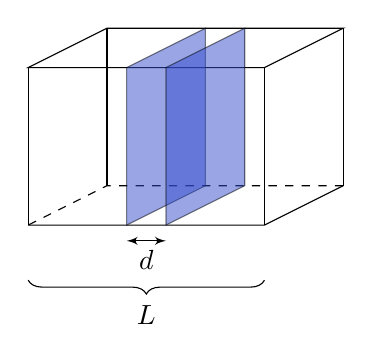
\begin{tikzpicture}
    \draw (0, 0) -- (3, 0) -- (4, 0.5);
    \draw [dashed] (4, 0.5) -- (1, 0.5) -- (0, 0);
    \draw (0, 2) -- (3, 2) -- (4, 2.5) -- (1, 2.5) -- cycle;
    \draw (0, 0) -- (0, 2);
    \draw (3, 0) -- (3, 2);
    \draw (1, 0.5) -- (1, 2.5);
    \draw (4, 0.5) -- (4, 2.5);

    \draw [fill=mblue, opacity=0.5] (1.25, 0) -- (2.25, 0.5) -- (2.25, 2.5) -- (1.25, 2) -- cycle;
    \draw [fill=mblue, opacity=0.5] (1.75, 0) -- (2.75, 0.5) -- (2.75, 2.5) -- (1.75, 2) -- cycle;

    \draw [latex'-latex'] (1.25, -0.2) -- (1.75, -0.2) node [pos=0.5, below] {$d$};

    \draw [decorate, decoration={brace, amplitude=5pt}] (3, -0.7) -- (0, -0.7);
    \node at (1.5, -0.9) [below] {$L$};
  \end{tikzpicture}
\end{center}
The presence of the plates means that the momentum of the field inside them is quantized
\[
  \mathbf{p} = \left(\frac{\pi n}{d}, p_y, p_z\right)
\]
for $n \in \Z$. For a massless scalar field, the energy per unit area between the plates is
\[
  E(d) = \sum_{n = 1}^\infty \int \frac{\d p_y\;\d p_z}{(2\pi)^2} \frac{1}{2} \sqrt{\left(\frac{\pi n}{d}\right)^2 + p_y^2 +p_z^2}.
\]
The energy outside the plates is then $E(L - d)$. The total energy is then
\[
  E = E(d) + E(L - d).
\]
This energy (at least naively) depends on $d$. So there is a force between the plates! This is the \emph{Casmir effect}, predicted in 1945, and observed in 1958. In the lab, this was done with the EM field, and the plates impose the boundary conditions.

Note that as before, we had to neglect modes with $|\mathbf{p}|$ too high. More precisely, we pick some distance scale $a \ll d$, and ignore modes where $|\mathbf{p}| \gg a^{-1}$. This is known as the ultraviolet cut-off. This is reasonable, since for high momentum modulus, we would break through the plates. Then we have
\[
  E(d) = A \sum_n \int \frac{\d p_y \;\d p_z}{(2\pi)^2} \frac{1}{2}|\mathbf{p}| e^{-a|\mathbf{p}|}.
\]
Note that as we set $a \to 0$, we get the previous expression.

Since we are scared by this integral, we consider the special case where we live in the $1 + 1$ dimensional world. Then this becomes
\begin{align*}
  E_{1 + 1}(d) &= \frac{\pi}{2d} \sum_{n = 1}^\infty n e^{-an\pi/d} \\
  &= -\frac{1}{2} \frac{\d}{\d a}\left(\sum_n e^{-an\pi/d}\right)\\
  &= -\frac{1}{2} \frac{\d}{\d a} \frac{1}{1 - e^{-a\pi/d}}\\
  &= \frac{\pi}{2d}\frac{e^{-a\pi/d}}{(1 - e^{-a\pi/d})^2}\\
  &= \frac{d}{2\pi a^2} - \frac{\pi}{24 d} + O(a^2).
\end{align*}
Our total energy is
\[
  E = E(d) + E(L - d) = \frac{L}{2\pi a^2} - \frac{\pi}{24}\left(\frac{1}{d} + \frac{1}{L - d}\right) + O(a^2).
\]
As $a \to 0$, this is still infinite, but the infinite term does not depend on $d$. The force itself is just
\[
  \frac{\partial E}{\partial d} = \frac{2\pi}{24 d^2} + O\left(\frac{d^2}{L^2}\right) + O(a^2),
\]
which is finite as $a \to 0$ and $L \to \infty$. So as we remove both the infrared and UV cutoffs, we still get a sensible finite force.

In $3 + 1$ dimensions, if we were to do the more complicated integral, it turns out we get
\[
  \frac{1}{A}\frac{\partial E}{\partial d} = \frac{\pi^2}{480 d^4}.
\]
The actual Casmir effect for electromagnetic fields is actually double this due to the two polarization states of the photon.

\subsection{Recovering particles}
It is easy to verify that
\[
  [H, a_\mathbf{p}^\dagger] = w_\mathbf{p} a_\mathbf{p}^\dagger
\]
and
\[
  [H, a_\mathbf{p}] = - \omega_\mathbf{p} a_\mathbf{p},
\]
which means (like SHO) we can construct energy eigenstates by acting with $a_\mathbf{p}^\dagger$. We let
\[
  \bket{\mathbf{p}} = a_\mathbf{p}^\dagger \bket{0}.
\]
Then we have
\[
  H\bket{\mathbf{p}} = \omega_\mathbf{p} \bket{\mathbf{p}},
\]
where the eigenvalue is
\[
  \omega_\mathbf{p}^2 = \mathbf{p}^2 + m^2.
\]
But from special relativity, we also know that the energy of a particle of mass $m$ and momentum $\mathbf{p}$ is given by
\[
  E_\mathbf{p}^2 = \mathbf{p}^2 + m^2.
\]
So we interpret $\bket{\mathbf{p}}$ as the momentum eigenstate of a particle of mass $m$ and momentum $\mathbf{p}$.

Note that in the Klein-Gordon field, we had
\[
  \mathcal{L} = \cdots + \frac{1}{2}m^2 \phi^2 + \cdots.
\]
So we can identify $m$ with the mass of the quantized particle. From now on, we will write $E_\mathbf{p}$ instead of $\omega_\mathbf{p}$.

Let's check this interpretation. After normal ordering, we have
\[
  \mathbf{P} = \int \pi(x) \nabla \phi(\mathbf{x}) \;\d^3 \mathbf{x} = \int \frac{\d^3 \mathbf{p}}{(2\pi)^3} \mathbf{p} a_\mathbf{p}^\dagger a_\mathbf{p}.
\]
So we have
\[
  \mathbf{P}\bket{\mathbf{p}} = \mathbf{p}\bket{\mathbf{p}}.
\]
So the state has total momentum $\mathbf{p}$.

We can also act with the angular momentum operator
\[
  J^i = \varepsilon^{ijk} \int \d^3 x\; (\mathcal{J}^a)^{jk},
\]
and obtain
\[
  J^i \bket{p} \to 0\text{ as }\mathbf{p} \to 0.
\]
So this particle has spin $0$. See example sheet $2$ for more details.

What about multi-particle states? We just have to act with more $a_\mathbf{p}^\dagger$'s. We have the $n$-particle state
\[
  \bket{\mathbf{p}_1, \cdots, \mathbf{p}_n} = a_{\mathbf{p}_1}^\dagger a_{\mathbf{p}_2}^\dagger \cdots a_{\mathbf{p}_n}^\dagger \bket{0}.
\]
Note that $\bket{\mathbf{p}, \mathbf{q}} = \bket{\mathbf{q}, \mathbf{p}}$ for any $\mathbf{p}, \mathbf{q}$. So any two parts are symmetric under interchange, ie. they are \term{bosons}.

The actual Hilbert space of particles is spanned by
\[
  \bket{0}, a_\mathbf{p}^\dagger \bket{0}, a_\mathbf{p}^\dagger, a_\mathbf{q}^{\dagger}\bket{0}, \cdots
\]
This is known as the \term{Fock space}. There is also an operator which counts the number of particles. It is
\[
  N = \int \frac{\d^3 \mathbf{p}}{(2\pi)^3} a_\mathbf{p}^\dagger a_\mathbf{p}.
\]
So we have
\[
  N\bket{\mathbf{p}_1, \cdots, \mathbf{p}_n} = n\bket{\mathbf{p}_1, \cdots, \mathbf{p}_n}.
\]
We have
\[
  [N, H] = 0
\]
So the particle number is conserved in the free theory. When we add interactions to the picture, this will no longer be the case.

Although we are calling these states ``particles'', they aren't localized --- they're momentum eigenstates. Theoretically, we can create a localized state via a Fourier transform:
\[
  \bket{\mathbf{x}} = \int\frac{\d^3 \mathbf{p}}{(2\pi)^3 e^{-i\mathbf{p}\cdot \mathbf{x}}}\bket{\mathbf{p}}.
\]
More generally, we can create a wave-packet, and insert $\psi(\mathbf{p}$ to get
\[
  \bket{\psi} = \int\frac{\d^3 \mathbf{p}}{(2\pi)^3 e^{-i\mathbf{p}\cdot \mathbf{x}}}\psi(\mathbf{p})\bket{\mathbf{p}}.
\]
Then this wave-packet can be both partially localized in space and in momentum.

For example, we can have
\[
  \psi(\mathbf{p}) = e^{-\mathbf{p}^2/2m}.
\]
Note now that neither $\bket{x}$ nor $\bket{\psi}$ are $H$-eigenstates, just like in non-relativistic quantum mechanics.

\subsection{Relativistic normalization}
We define the vacuum such that $\braket{0}{0} = 1$, and the $1$-particle state $\bket{\mathbf{p}} = a_\mathbf{p}^\dagger \bket{0}$, which satisfies
\[
  \braket{\mathbf{p}}{\mathbf{q}} = (2\pi)^3 \delta^3(\mathbf{p} - \mathbf{q}).
\]
Is this equation Lorentz invariant? It is not obvious, because we are writing in $3$-vectors.

What could go wrong with Lorentz invariance? Suppose we have a Lorentz transformation
\[
  p^\nu \mapsto \Lambda^\mu\!_\nu p^\nu = p'^\mu.
\]
We want the states $\bket{\mathbf{p}}$ and $\bket{\mathbf{p}'}$ to be related by some unitary transformation $U(\Lambda)$. But we haven't been careful about normalization. So there is no reason why we would get a unitary transformation.

The trick to figuring out the normalization is by looking at an object we know is Lorentz invariant. For example, the identity operator on a 1-particle state given by
\[
  1 = \int \frac{\d^3 \mathbf{p}}{(2\pi)^3} \bket{\mathbf{p}} \brak{\mathbf{p}}.
\]
Individually, we know $\frac{\d^3 \mathbf{p}}{(2\pi)^3}$ and $\bket{\mathbf{p}}\brak{\mathbf{p}}$ are not Lorentz invariant, but they are when put together, because $1$ is.

\begin{prop}
  The expression
  \[
    \int \frac{\d^3 \mathbf{p}}{2 E_p}
  \]
  is Lorentz-invariant.
\end{prop}

\begin{proof}
  Indeed, we know $\int \d^4 p$ certainly is Lorentz invariant, and the relativistic dispersion relation for particles of mass $m$ is
  \[
    p_0^2 = E_\mathbf{p}^2 = \mathbf{p}^2 + m^2,
  \]
  where $\mathbf{p}$ is the $3$-momentum. This is again Lorentz invariant. The solutions for $p_0$ have $2$ branches $p_0 = \pm E_\mathbf{p}$, but the choice of branch is Lorentz invariant, ie. we can change from the positive energy to a negative energy by doing a Lorentz boost. So the following combination is Lorentz invariant:
  \[
    \int \d^4 p\; \delta(p_0^2 - \mathbf{p}^2 - \mathbf{m}^2).
  \]
  Using the properties of the Dirac delta function, this is equal to
  \[
    \int \frac{\d^3 \mathbf{p}}{2 p_0} = \int \frac{\d^3 \mathbf{p}}{2 E_p}.
  \]
\end{proof}

Thus, we have
\begin{prop}
  The expression
  \[
    2E_\mathbf{p} \delta^3 (\mathbf{p} - \mathbf{q})
  \]
  is Lorentz invariant.
\end{prop}

\begin{proof}
  We have
  \[
    \int \frac{\d^3 \mathbf{p}}{2 E_\mathbf{p}} \cdot (2E_\mathbf{p} \delta^3(\mathbf{p} - \mathbf{q})) = 1.
  \]
  Since the RHS is Lorentz invariant, and the measure is Lorentz invariant, we know $2E_\mathbf{p} \delta^3(\mathbf{p} - \mathbf{q})$ must be Lorentz invariant.
\end{proof}

From this, we learn that the correctly normalized states are
\[
  \bket{p} = \sqrt{2 E_\mathbf{p}}\bket{\mathbf{p}} = \sqrt{2 E_\mathbf{p}} a_\mathbf{p}^\dagger \bket{0}.
\]
These new states satisfy
\[
  \braket{p}{q} = (2\pi)^3 (2E_\mathbf{p}) \delta^3 (\mathbf{p} - \mathbf{q}),
\]
and is Lorentz invariant.

We can then rewrite the identity as
\[
  1 = \int \frac{\d^3 \mathbf{p}}{(2\pi)^3}\frac{1}{2 E_\mathbf{p}} \bket{p}\brak{p}.
\]
We can now define relativistically normalized creation operators by
\[
  a^\dagger(p) = \sqrt{2E_\mathbf{p}} a_\mathbf{p}^\dagger.
\]
Then we can write our field as
\[
  \phi = \int \frac{\d^3 \mathbf{p}}{(2\pi)^3}\frac{1}{2E_\mathbf{p}} e^{i\mathbf{p}\cdot \mathbf{x}}(a^\dagger(p) + a(p)).
\]
\subsection{Complex scalar fields}
Consider a complex Lagrangian
\[
  \mathcal{L} = \partial_\mu \psi^* \partial^\mu \psi - \mu^2 \psi^* \psi.
\]
The Euler-Lagrange equations then say
\begin{align*}
  \partial_\mu \partial^\mu \psi + \mu^2 \psi &= 0\\
  \partial_\mu \partial^\mu \psi^* + \mu^2 \psi^* &= 0
\end{align*}
Note that the second equation is just the complex conjugate of the first.

Since $\psi$ is not equal to $\psi^\dagger$, we need a more complicated expression for $\psi$ in terms of creation and annihilation operators.
\[
  \psi = \int \frac{\d^3 \mathbf{p}}{(2\pi)^3}\frac{1}{\sqrt{2 E_\mathbf{p}}}(b_\mathbf{p} e^{i \mathbf{p}\cdot \mathbf{x}} + C_\mathbf{p}^\dagger e^{-\mathbf{p}\cdot \mathbf{x}}).
\]
So we have
\[
  \psi^\dagger = \int \frac{\d^3 \mathbf{p}}{(2\pi)^3} \frac{1}{\sqrt{2E_\mathbf{p}}} (b_\mathbf{p}^\dagger e^{-i\mathbf{p}\cdot \mathbf{x}} + C_\mathbf{p} e^{i\mathbf{p}\cdot \mathbf{x}}).
\]
Then the energy momentum is
\[
  \pi = \frac{\partial \mathcal{L}}{\partial \dot{\psi}} = \dot{\psi}^* = \int \frac{\d^3 \mathbf{p}}{(2\pi)^3} \sqrt{\frac{E_\mathbf{p}}{2}} (b_\mathbf{p}^\dagger e^{-i\mathbf{p}\cdot \mathbf{x}} - C_\mathbf{p}e^{i\mathbf{p}\cdot \mathbf{x}})
\]
So we have
\[
  \pi^\dagger = \int \frac{\d^3 \mathbf{p}}{(2\pi)^3}(-i) \sqrt{\frac{E_\mathbf{p}}{2}} (b_\mathbf{p} e^{i\mathbf{p}\cdot \mathbf{x}} - C_\mathbf{p}^\dagger e^{i\mathbf{p}\cdot \mathbf{x}}).
\]
The commutator relations are
\[
  [\psi(\mathbf{x}), \pi(\mathbf{y})] = i \delta^3(\mathbf{x} - \mathbf{y}),\quad [\psi(\mathbf{x}) \pi^\dagger(\mathbf{y})] = 0,\quad\cdots,
\]
and these are equivalent to
\[
  [b_\mathbf{p}, b_\mathbf{q}^\dagger] = (2\pi)^3 \delta^3(\mathbf{p} - \mathbf{q}),\quad [c_\mathbf{p}, c_\mathbf{q}^\dagger] = (2\pi)^3 \delta^3(\mathbf{p} - \mathbf{q}),
\]
with all other commutators zero.

Recall that this theory has a conserved charge. Classically, this is given by
\[
  Q = i \int \d^3 \mathbf{x} (\dot{\psi}^* \psi - \psi^* \dot{\psi}) = i \int \d^3 \mathbf{x} (\pi \psi - \psi^* \pi^*).
\]
The claim is that (after normal ordering)
\[
  Q = \int \frac{\d^3 \mathbf{p}}{(2\pi)^3} c_\mathbf{p}^\dagger c_\mathbf{p} - b_\mathbf{p}^\dagger b_\mathbf{p} = N_c - N_b,
\]
where $N_C$ counts the number of $C$ particles and $N_b$ count the number of $b$ particles. They both have spin $0$ and mass $\mu$. So we can interpret these as particles and anti-particles.

Looking back, for a real scalar field, the particle is equal to the antiparticle.

It is easy to compute
\[
  [Q, H] = 0.
\]
So we see that $Q$ is conserved. This is not a big deal, since $N_c$ and $N_b$ are separately conserved. However, in the interacting theory, they are \emph{not} separately conserved, but $Q$ still is.

\subsection{The Heisenberg picture}
Although our theory is Lorentz invariant, it is not so obvious. For example, $\phi$ depends on $\mathbf{x}$, but not on $t$, and the states evolve in $t$ by the Schr\"odinger equation
\[
  i \frac{\d}{\d t}\bket{\mathbf{p}} = H\bket{\mathbf{p}} = E_\mathbf{p} \bket{\mathbf{p}}.
\]
We can solve this easily to see that
\[
  \bket{\mathbf{p}(t)} = e^{-iE_\mathbf{p} t} \bket{\mathbf{p}(0)}.
\]
Things look better in the Heisenberg picture, where we put the time dependence in the operators:
\[
  O_H(t) = e^{iHt} O_S e^{iHt},
\]
where $O_S$ is an operator in the Schr\"odinger picture, and $O_H$ is the corresponding operator in the Heisenberg picture. We then find that
\[
  \frac{\d O_H}{\d t} = i [H, O_H].
\]
These agree at $t = 0$. In this language, the operators satisfy equal time commutation relations
\[
  [\phi(\mathbf{x}, t), \phi(\mathbf{y}, t)] = [\pi(\mathbf{x}, t), \pi(\mathbf{y}, t)] = 0,\quad [\phi(\mathbf{x}, t), \psi(\mathbf{y}, t)] = i \delta^3(\mathbf{x} - \mathbf{y}).
\]
We can check that if we write $O_H = \phi$, then the equation means that the Heisenberg operator $\phi$ satisfies the Klein-Gordon equation
\[
  \partial_\mu \partial^\mu \phi + m^2 \phi = 0.
\]
We write the Fourier transform of $\phi(x)$ by using
\[
  e^{iHt}a_\mathbf{p} e^{-iHt} = e ^{-iE_\mathbf{p} t}a_\mathbf{p},
\]
using
\[
  [H, a_\mathbf{p}] = -E_\mathbf{p} a_\mathbf{p},
\]
and similarly
\[
  e^{iHt} a_\mathbf{p}^\dagger e^{iHt} e^{iE_\mathbf{p} t} a_\mathbf{p}^\dagger.
\]
So we have
\[
  \phi(\mathbf{x}, t) = \int \frac{\d^3 \mathbf{p}}{(2\pi)^3}\frac{1}{2 E_\mathbf{p}} \left(a_\mathbf{p} e^{-ip \cdot x} + a_\mathbf{p}^\dagger e^{i p \cdot x}\right).
\]
Note that we have replaced $\mathbf{p}\cdot \mathbf{x}$ with $p \cdot x$, since we had an extra factor of $e^{-iE_p t}$ from conjugating by $e^{iHt}$.

\subsection{Causality}
We started with a Lorentz-invariant Lagrangian, and slowly butchered it as we picked a preferred time direction. While the Heisenberg picture makes it look a bit more Lorentz invariant, it still had the problem of obeying equal time commutation relations, ie. we required
\[
  [\phi(\mathbf{x}, t) = \pi(\mathbf{y}, t)] = i \delta^3(\mathbf{x} - \mathbf{y}).
\]
What about arbitrary space-time separations? In particular, causality requires that all space-like separated operators commute, ie.
\[
  [O(x), O(y)] = 0
\]
for all $(x - y)^2 < 0$. This ensures that a measurement at $x$ cannot affect a measurement at $y$. Do we have it?

We define
\[
  \Delta(x - y) = [\phi(x), \phi(y)].
\]
We then have
\[
  \Delta(x - y) = \int \frac{\d^3 p}{(2\pi)^3} \frac{1}{2 E_p} \left(e^{i p \cdot(x - y)} - e^{ip \cdot (x - y)}\right).
\]
Note that the right hand side is an operator, while the left hand side is just an ordinary function, ie. a \term{c-function}. What do we know about this function? We know it is Lorentz invariant, since $\int \frac{\d^3p}{2 E_p}$ is Lorentz invariant, and so are the integrands.

This \emph{doesn't} vanish for time-like separation, since we have
\[
  [\phi(\mathbf{x}, 0), \phi (\mathbf{x}, t)] \propto e^{-imt} - e^{imt}.
\]
but it does for space-like separation. We note that
\[
  \Delta (x, y) = 0
\]
at equal times, but is Lorentz invariant. So it can only depend on the combination $(x - y)^2$. So if it vanishes at equal times (when $x \not= y$), it must vanish for all $(x - y)^2 < 0$.

So this theory is causal.

Note that we have
\[
  [\phi(\mathbf{x}, t), \phi(\mathbf{y}, t)] = \frac{1}{2}\int \frac{\d^3 \mathbf{p}}{(2\pi)^3} \frac{1}{\sqrt{\mathbf{p}^2 + m^2}} \left(e^{i\mathbf{p}\cdot (\mathbf{x} - \mathbf{y})} - e^{-i\mathbf{p}\cdot (\mathbf{x} - \mathbf{y})}\right).
\]
When $\mathbf{x} \not= \mathbf{y}$, we can change the sign of the $\mathbf{p}$ in the second $e^{-i\mathbf{p}\cdot (\mathbf{x} - \mathbf{y})}$, since we are integrating over all possible momentum. So the two terms cancel, and the result vanishes.

This will also hold in an interacting theory.

\section{Propagators}
We want to ask the question: if we prepare a particle at $y$, what is the probability amplitude of finding it at a point $x$? In the case of a scalar field theory, we know what to do --- we have
\[
  \brak{0}\phi(x) \phi(y) \bket{0} = \int \frac{\d^3 \mathbf{p}}{(2\pi)^3} \frac{\d^3 \mathbf{p}'}{(2\pi)^3} \frac{1}{\sqrt{4E_\mathbf{p} E_\mathbf{p}'}} \brak{0}a_\mathbf{p} a_{\mathbf{p}'}^\dagger \bket{0} e^{-i p \cdot x + i p' \cdot y}.
\]
We now use the fact that
\[
  \brak{0}a_\mathbf{p}, a_\mathbf{p}^\dagger\bket{0} = \brak{0}[a_\mathbf{p}, a_\mathbf{p}^\dagger]\bket{0} = i (2\pi)^3 \delta^3 (\mathbf{p} - \mathbf{p}'),
\]
since $a_\mathbf{p}^\dagger a_\mathbf{p} \bket{0} = 0$. So we have
\[
  \brak{0} \phi(x) \phi(y) \bket{0} = \int \frac{\d^3 \mathbf{p}}{(2\pi)^3} \frac{1}{2 E_\mathbf{p}} e^{i p \cdot (x - y)}.
\]
We call this $D(x - y)$, the \term{propagator}.

For space-like separation $(x - y)^2 < 0$, one can show that it decays as
\[
  D(x - y) \sim e^{-m(|\mathbf{x} - \mathbf{y}|)}.
\]
Note that this is non-vanishing! So we see that the quantum field leaks outside the light cone a bit. However, we have just seen that space-like measurements commute. We know that
\[
  \Delta(x - y) = [\phi(x), \phi(y)] = D(x - y) - D(y - x),
\]
and this is $0$ if $(x - y)^2 < 0$.

Note that when $(x - y)^2 < 0$, there is no Lorentz-invariant way to order the events. If a particle can travel in a spacelike direction $\mathbf{x} \to \mathbf{y}$, it can just as easily travel in the other direction. In a measurement, these two amplitudes cancel. So we are fine.

With a complex scalar field, we get something more interesting. We have
\[
  [\psi(x), \psi^\dagger(y)] = 0
\]
outside the light cone. The interpretation now is that the propagation of the particle from $\mathbf{x} \to \mathbf{y}$ cancels the propagation of the antiparticle in the opposite direction.

\subsection{Feynman propagator}

We are now going to introduce one of the most important propagators in quantum field theory:
\begin{defi}[Feynman propagator]\index{Feynman propagator}
  The \emph{Feynman propagator} is
  \[
    \Delta_F (x - y) = \brak{0} T \phi(x) \phi(y) \bket{0} =
    \begin{cases}
      \brak{0} \phi(x) \phi(y) \bket{0} & x^0 > y^0\\
      \brak{0} \phi(y) \phi(x) \bket{0} & y^0 > x^0
    \end{cases}
  \]
\end{defi}

\begin{prop}
  We have
  \[
    \Delta_F = \int \frac{\d^4 p}{(2\pi)^4 } \frac{i}{p^2 - m^2} e^{-ip \cdot (x - y)}.
  \]
  This expression is a priori ill-defined since for each $\mathbf{p}$, the integrand over $p^0$ has a pole whenever $(p^0)^2 = \mathbf{p}^2 + m^2$. So we need a prescription for avoiding this. We replace this with a complex contour integral with contour given by
  \begin{center}
    \begin{tikzpicture}
      \draw [->] (-4, 0) -- (4, 0);
      \draw [->] (0, -2) -- (0, 2);

      \node [circ] at (-2, 0) {};
      \node [above] at (-2, 0) {$-E_\mathbf{p}$};
      \node [circ] at (2, 0) {};
      \node [below] at (2, 0) {$E_\mathbf{p}$};

      \draw [thick, blue] (-4, 0) -- (-2.5, 0) arc (180:360:0.5) -- (1.5, 0) arc(180:0:0.5) -- (4, 0);
    \end{tikzpicture}
  \end{center}
  Writing
  \[
    \frac{1}{p^2 - m^2} = \frac{1}{p_0^2 - E_\mathbf{p}^2} = \frac{1}{(p^0 - E_\mathbf{p})(p^0 + E_\mathbf{p})},
  \]
  we see that the residue of the pole at $p^0 = \pm E_\mathbf{p}$ is $\pm \frac{1}{2E_\mathbf{p}}$.

  When $x^0 > y^0$, we close the contour in the lower plane $p^0 \to -i\infty$, so $e^{-p^0(x^0 - t^0)} \to e^{-\infty} = 0$. Then $\int p^0$ picks up the residue at $p^0 = E_\mathbf{p}$. So the Feynman propagator is
  \begin{align*}
    \Delta_F (x - y) &= \int \frac{\d ^3 \mathbf{p}}{(2\pi)^4} \frac{(-2\pi i)}{2E_\mathbf{p}} i e^{-iE_\mathbf{p}(x^0 - y^0) + i \mathbf{p} (\mathbf{x} - \mathbf{y})}\\
    &= \int \frac{\d^3 \mathbf{p}}{(2\pi^3)} \frac{1}{2 E_\mathbf{p}} e^{-ip \cdot (x - y)}.
  \end{align*}
  When $x^0 < y^0$, we close the contour in the upper-half plane. Then we have
  \begin{align*}
    \Delta_F(x - y) &= \int \frac{\d^3 \mathbf{p}}{(2\pi)^4} \frac{2\pi i}{-2E_\mathbf{p}} i e^{iE_\mathbf{p} (x^0 - y^0) + i\mathbf{p} \cdot (\mathbf{x} - \mathbf{y})}\\
    &= \int \frac{\d^3 \mathbf{p}}{(2\pi)^3} \frac{1}{2E_\mathbf{p}} e^{-i E_\mathbf{p}(y^0 - x^0) - i \mathbf{p}\cdot (\mathbf{y} - \mathbf{x})}\\
    \intertext{We again use the trick of flipping the sign of $\mathbf{p}$ to obtain}
    &= \int \frac{\d^3 \mathbf{p}}{(2\pi)^3} \frac{1}{2E_\mathbf{p}} e^{-ip\cdot(y - x)}.
  \end{align*}
  Instead of specifying the contour, we write
  \[
    \Delta_F(x - y) = \int \frac{\d^4 p}{(2\pi)^4} \frac{i e^{-ip\cdot(x - y)}}{p^2 - m^2 + i \varepsilon},
  \]
  where $\varepsilon$ is taken to be small, or infinitesimal. This is known about the ``$i\varepsilon$-prescription''. Then the poles are shifted slightly away from the real axis, and we can just integrate along the real axis.
\end{prop}
The propagator is in fact the Green's function of the Klein-Gordon operator:
\begin{align*}
  (\partial_t^2 - \nabla^2 + m^2) \Delta_F(x - y) &= \int \frac{\d^4 p}{(2\pi)^4} \frac{i}{p^2 - m^2}(-p^2 + m^2) e^{-ip\cdot(x - y)}\\
  &= -i \int \frac{\d^4 p}{(2\pi)^4} e^{-ip\cdot(x - y)}\\
  &= -i \delta^4(x - y).
\end{align*}
Note that this didn't use the contour!

\subsection{Other propagators}
For some purposes, it's useful to pick other contours, eg. the \term{retarded Green's function} defined as follows:
\begin{center}
  \begin{tikzpicture}
    \draw [->] (-4, 0) -- (4, 0);
    \draw [->] (0, -2) -- (0, 2);

    \node [circ] at (-2, 0) {};
    \node [below] at (-2, 0) {$-E_\mathbf{p}$};
    \node [circ] at (2, 0) {};
    \node [below] at (2, 0) {$E_\mathbf{p}$};

    \draw [thick, blue] (-4, 0) -- (-2.5, 0) arc (180:0:0.5) -- (1.5, 0) arc(180:0:0.5) -- (4, 0);
  \end{tikzpicture}
\end{center}
This can be given in terms of operators by
\begin{defi}[Retarded Green's function]
  The \emph{retarded Green's function} is given by
  \[
    \Delta_R(x - y) =
    \begin{cases}
      [\phi(x), \phi(y)]& x^0 > y^0\\
      0 & y^0 > x^0
    \end{cases}
  \]
\end{defi}
This is useful if we have some initial field configuration, and we want to see how it evolves in the presence of some source. This solves the ``inhomogeneous Klein-Gordon equation'', ie. an equation of the form
\[
  \partial_\mu \partial^\mu + m^2 \phi = J(x),
\]
where $J(x)$ is some background function.

One also defines the \term{advanced Green's function} which vanishes when $y^0 < x^0$ instead. This is useful if we know the end-point of a field configuration and want to know where it came from. However, in general, the Feynman propagator is the most useful in quantum field theory.

\section{Interacting fields}
Free theories are special --- we can determine the exact spectrum, but nothing interacts. These facts are related. Free theories have at most quadratic terms in the Lagrangian. So the equations of motion are linear. So we get exact quantization, and we get multi-particle states with no interactions by superposition.

Let's add interaction terms to the Lagrangian --- higher powers of the fields. We want to apply perturbation theory to the system, so we will consider cases where the interactions are \emph{small}. For example, for a real scalar field $\phi$, we can have a Lagrangian
\[
  \mathcal{L} = \frac{1}{2} \partial_\mu \phi \partial^\mu \phi - \frac{1}{2}m^2 \phi^2 - \sum_{n = 3}^\infty \frac{\lambda_n}{n!} \phi^n.
\]
The constants $\lambda_n$ are the \term{coupling constants}. Recall that $[S] = 0$, and $S = \int \d^4 x \mathcal{L}$. Since $[d^4 x] = -4$, we have $[\mathcal{L}] = 4$.
Since $[\partial_\mu] = 1$, we know from the $\partial_\mu \phi \partial^\mu \phi$ term that $[\phi] = 1$. Finally, from the $m^2 \phi^2$ term, we have $[m] = 1$, as expected. From this, we deduce that $[\lambda_n] = 4 - n$.

Now which terms are ``small''? We would like to say that $\lambda_n \ll 1$, but this only makes sense if our quantities are dimensionless.

Here there are three classes of terms:
\begin{enumerate}
  \item $[\lambda_3] = 1$. If we have some energy scale $E$ for what is going on around us, then we have a dimensionless parameter $\frac{\lambda_3}{E}$. So $\lambda^3 \phi^3/3!$ is a small perturbation at high energies, and large perturbations at low energies.

    This in fact happens in reality, as we have a term like this in the standard model for couplings of the Higgs boson.

    Such perturbations are called \term{relevant perturbation}\emph{s} at low energies. In a relativistic theory, we have $E > m$. So we can always make the perturbation small by picking $\lambda_3 \ll m$, at least when we are working with general theory.

  \item $[\lambda_4] = 0$. This is dimensionless. So this is small $\lambda_4 \ll 1$. This is known as \term{marginal perturbation}.

  \item For all $n > 4$, this has dimensionless parameter $\lambda_n E^{n - 4}$. This is small at low energies, and high at large energies. These operators are called \term{irrelevant perturbation}\emph{s}.
\end{enumerate}
While we call them ``irrelevant'', they are indeed relevant, as it is typically difficult to avoid high energies in quantum field theory. Indeed, we have seen that we can have arbitrarily large vacuum fluctuations. We might then expect problems with these irrelevant operators. These are technically non-renormalizable theories. See Advanced Quantum Field Theory for more.

In this course, we will consider only weakly coupled field theories --- one that can truly be considered as small perturbations of the free theory at all energies.

\begin{eg}[$\phi^4$ theory]\index{$\phi^4$ theory}
  Consider the $\phi^4$ theory
  \[
    \mathcal{L} = \frac{1}{2} \partial_\mu \phi \partial^\mu \phi - \frac{1}{2}m^2 \phi^2 - \frac{\lambda}{4!}\phi^4,
  \]
  where $\lambda \ll 1$. We can already guess the effects of the final term by noting that here we have
  \[
    [H, N] \not= 0.
  \]
  So particle number is \emph{not} conserved. Expanding the last term in the Lagrangian in terms of $a_\mathbf{p}, a_\mathbf{p}^\dagger$, we get terms involving things like $a_\mathbf{p} a_\mathbf{p} a_\mathbf{p} a_\mathbf{p}$ or $a_\mathbf{p}^\dagger a_\mathbf{p}^\dagger a_\mathbf{p}^\dagger a_\mathbf{p}^\dagger$ or $a_\mathbf{p}^\dagger a_\mathbf{p}^\dagger a_\mathbf{p}^\dagger a_\mathbf{p}$, and all other combinations you can think of. These will create or destroy particles.
\end{eg}

\begin{eg}[Scalar Yukawa theory]\index{scalar Yukawa theory}
  In the early days, we found things called \emph{pions} that seemed to mediate nuclear reactions. At that time, people did not know that things are made up of quarks. So they modelled these pions in terms of scalar field, and we have
  \[
    \mathcal{L} = \partial_\mu \psi^* \partial^\mu \psi + \frac{1}{2} \partial_\mu \phi \partial^\mu \phi - M^2 \psi^* \psi - \frac{1}{2} m^2 \phi^2 - g \psi^* \psi \phi.
  \]
  Here we have $g \ll m, M$. Here we still have $[Q, H] = 0$, as all terms are at most quadratic in the $\psi$'s. So the number of $\psi$-particles minus the number of $\psi$-antiparticles is still conserved. However, there is no particle conservation for $\phi$.

  A wary --- the potential
  \[
    V = M^2 \psi^* \psi + \frac{1}{2} m \phi^2 + g \psi^*\psi \phi
  \]
  has a stable local minimum when the fields are zero, but it is unbounded below for large $-g \phi$. So we can't push the theory too far.
\end{eg}
The study of strongly coupled field theories is a major research topic in quantum field theory. In some particular solids, we can get charge fractionalization --- Solids contain electrons, and each has $\pm 1$ charges. However, in complicated systems, we can get excitations with fractional charges, and this gives the fractional quantum hall effect. Another topic people study is confinement. We want to figure out what quarks and gluons are always stuck together in mesons and baryons at lower energies. Another issue is emergent gravity --- there are some theories in four dimensions that are somehow equivalent to 10-dimensional quantum gravity. This is known as the \term{AdS/CFT correspondence}, standing for anti-de Sitter space and conformal field theory.

\section{Interaction picture}
The \emph{interaction picture} is a mixture of the Schr\"odinger picture and the Heisenberg picture, where the simple time evolutions remain in the states, whereas the complicated interactions live in the operators. This is a very useful trick if we want to deal with small interactions.

Recall that in the Schr\"odinger picture, the states evolve with $t$, satisfying
\[
  i \frac{\partial}{\partial t}\bket{\psi}_S = H \bket{\psi}_S,
\]
while the operators $O_s$ are time independent.

In the Heisenberg picture, the states are fixed but the operators evolve in time, and the operators are rleated by
\[
  O_H(t) = e^{iHt}O_s e^{-iHt},
\]
while
\[
  \bket{\psi}_H = e^{iHt}\bket{\psi}_S.
\]
The interaction picture is a hybrid of the two. We split the Hamiltonian up as
\[
  H = H_0 + H_{int}.
\]
The time dependence of operators is governed by $H_0$, whereas the time dependence of states is controlled by $H_{int}$. Of course, at this moment, this split is arbitrary, but it is useful if we make the right choices. We will choose $H_0$ to be very simple (eg. a free field theory), and this will make our life easy.
\[
  \bket{\psi}_I = e^{iH_0 t} \bket{\psi(t)}_S, \quad O_I(T) = e^{iH_0 t} O_S e^{-iH_0 t}.
\]
Then we have
\[
  H_I = (H_{int})_I = e^{iH_0 t} H_{int} e^{iH_0 t}.
\]
What is the right equation of motion? The Schr\"odinger equation is
\[
  i \frac{\d \bket{\psi}_S}{\d t} = H_S \bket{\psi}_S.
\]
Putting in our definitions, we have
\[
  i \frac{\d}{\d t}(e^{-iH_0 t}\bket{\psi}_i) = (H_0 + H_{int})_S e^{-iH_0 t} \bket{\psi}_I.
\]
Writing this out and using the chain rule, we are left with
\[
  i \frac{\d \bket{\psi}_I}{\d t} = e^{iH_0 t} H_{int} e^{-iH_0 t} \bket{\psi}_I.\tag{$*$}
\]
We write
\[
  H_I(t) = e^{iH_0 t} H_{int} e^{-iH_0 t} \bket{\psi}_I.
\]
\emph{Dyson's formula} tells us to do this: Let's try a solution to $(*)$ given by
\[
  \bket{\psi(t)}_I = U(t, t_0) \bket{\psi(t_0)}_I,
\]
where $U(t, t_0)$ is the unitary time evolution operator satisfying
\[
  U(t_1, t_2) U(t_2, t_3) = U(t_1, t_3),\quad U(t, t) = 1.
\]
Then we have
\[
  i \frac{\d U}{\d t} = H_I(t) U.
\]
If $H_I$ were an ordinary function, we could solve this by
\[
  U(t, t_0) = \exp\left(-i \int_{t_0}^t H_I(t') \;\d t'\right).
\]
But the trouble is that $H_I$ is an operator, and we have ordering ambiguities, since
\[
  [H_I(t'), H_I(t'')] \not= 0
\]
for $t' \not= t''$. So what we do is to take that solution as an idea, and order them appropriately.
\begin{prop}[Dyson's formula]\index{Dyson's formula}
  The solution to the Schr\"odinger equation in the interaction picture is given by
  \[
    U(t, t_0) = T\exp\left(-i \int_{t_0}^t H_I(t') dt'\right),
  \]
  where $T$ stands for \term{time ordering}: operators evaluated at earlier times appear on the RHS when we write out the power series. More explicitly,
  \[
    T\{O_1(t_1) O(t_2)\} =
    \begin{cases}
      O_1(t_1) O_2(t_2) & t_1 > t_2\\
      O_2(t_2) O_1(t_1) & t_2 > t_1
    \end{cases}.
  \]
  We do not specify what happens when $t_1 = t_2$, but it doesn't matter in our case since the operators are then equal.

  Thus, we have
  \begin{multline*}
    U(t, t_0) = 1 - i \int_{t_0}^t H_I (t') \d t' + \frac{(-i)^2}{2} \left\{\int_{t_0}^t \d t' \int_{t'}^t H_I(t'') H_I(t')\right.\\
    \left.+ \int_{t_0}^t \d t' \int_{t_0}^{t'} \d t''\; H_I(t') + H_I(t'')\right\} + \cdots.
  \end{multline*}
  We now notice that a simple relabelling shows that the last two terms are actually the same thing. So we have
  \[
    U(t, t_0) = 1 - i \int_{t_0}^t H_I (t') \d t' + (-i)^2 \int_{t_0}^t \d t' \int_{t'}^t \d t'' \; H_I(t'') H_I(t') + \cdots.
  \]
\end{prop}

\begin{proof}
  Under this time ordering, all operators commute, since their order is already fixed. So we have
  \begin{align*}
    i\frac{\d}{\d t}\left(T\exp\left(-i \int_{t_0}^t \d t'\; H_I (t')\right)\right) &= T\left(H_I(t) \exp\left(-i \int_{t_0}^t \d t' H_I(t')\right)\right)\\
    &= H_I(t_0) T \exp\left(-i \int_{t_0}^t H_I(t')\right).
  \end{align*}
  This works because $t$ is on the upper limit of the integral is the latest time, so we can pull $H_I(t)$ to the LHS.
\end{proof}
This result isn't too practically useful, since the time-ordered exponential is typically very difficult to compute. However, if we work with small perturbations, we can just use the power series and take the first few terms.

\subsection{A first look at scattering}
We are now going to apply the interaction picture to QFT, starting with
\[
  H_{int} = g\psi^* \psi \phi
\]
We can expand $\phi$ in terms of the creation and annihilation operators $a$ and $a^\dagger$. We will use this to describe the creation and destruction of mesons.

Similarly, we can expand $\psi$ in terms $b$ and $c^\dagger$, which destroys a particle, or creates an antiparticle, and $\psi^*$ can be expanded in terms of $b^\dagger$ and $c$. We imagine that the particles represented by $\psi$ are nucleons.

Recall that the particle number is not conserved, but the charge $Q = N_c - N_b$ is.

At first order in perturbation theory, we have terms like $b^\dagger c^\dagger a$. This destroys a meson and produces a $\psi \bar{\psi}$ pair (where $\bar{\psi}$ is the anti-$\psi$). This contributes to meson decay $\phi \to \psi + \bar{\psi}$.

We can draw a picture of this:
\begin{center}
  \begin{tikzpicture}
    \draw [->-=0.6] (0, 0) node [left] {$\phi$} -- (1.5, 0);
    \draw [->-=0.6] (1.5, 0) -- (3, 1) node [right] {$\psi$};
    \draw [->-=0.6] (1.5, 0) -- (3, -1) node [right] {$\bar{\psi}$};
  \end{tikzpicture}
\end{center}
At second order in perturbation theory, we have more complicated terms like $(c^\dagger b^\dagger a)(cba^\dagger)$. This gives rise to a scattering process
\[
  \psi + \bar{\psi} \to \phi \to \psi + \bar{\psi}.
\]
\begin{center}
  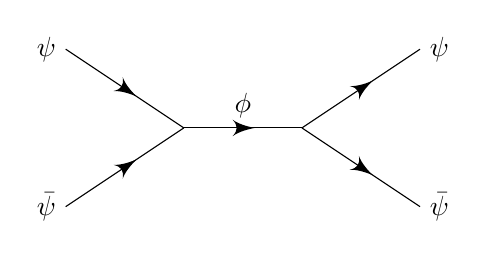
\begin{tikzpicture}
    \draw [->-=0.6] (-1.5, 1) node [left] {$\psi$} -- (0, 0);
    \draw [->-=0.6] (-1.5, -1) node [left] {$\bar{\psi}$} -- (0, 0);
    \draw [->-=0.6] (0, 0) -- (1.5, 0) node [pos=0.5, above] {$\phi$};
    \draw [->-=0.6] (1.5, 0) -- (3, 1) node [right] {$\psi$};
    \draw [->-=0.6] (1.5, 0) -- (3, -1) node [right] {$\bar{\psi}$};
  \end{tikzpicture}
\end{center}
To calculate the amplitudes, we will make an important assumption that the particles do not interact before and after the scattering, and they behave like free particles. This means the initial state $\bket{i}$ at $t \to -\infty$ and the final state $\bket{f}$ at $t \to \infty$ are eigenstates of the free Hamiltonian $H_0$ and the particle number $N$. It's plausible since at $t = \pm \infty$, the states are well-separated in space, and they don't feel the effect of each other.

As the paths approach each other, they interact before departing again, each going on its own way. The amplitude to go from $\bket{i} \to \bket{f}$ is
\[
  \lim_{t_{\pm} \to \pm \infty} \brak{f} O(t_+, t_-) \bket{i} \equiv \brak{f}S\bket{i}.
\]
The operator $S$ is a unitary operator known as the \term{$S$-matrix}, for ``scattering''.

There are some caveats with the assumption that they initial and final states do not interact, and sometimes we have to deal with these separately. For example, if we want to break up a proton to see what is going on in there, we certainly do not have an initial free state.

The bound states show up as poles in the $S$-matrix.

\begin{eg}
  We want to find the probability of
  \begin{center}
    \begin{tikzpicture}
      \draw [->-=0.6] (0, 0) node [left] {$\phi$} -- (1.5, 0);
      \draw [->-=0.6] (1.5, 0) -- (3, 1) node [right] {$\psi$};
      \draw [->-=0.6] (1.5, 0) -- (3, -1) node [right] {$\bar{\psi}$};
    \end{tikzpicture}
  \end{center}
  happening. We have
  \begin{align*}
    \bket{i} = \sqrt{2E_\mathbf{p}} a_\mathbf{p}^\dagger \bket{0}\\
    \bket{f} = \sqrt{4E_{\mathbf{q}_1} E_{\mathbf{q}_2}} b_{\mathbf{q}_1}^\dagger c_{\mathbf{q}_2}^{\dagger} \bket{0}.
  \end{align*}
  The transition corresponds to the $c^\dagger b^\dagger a$ term. We then have
  \begin{align*}
    \brak{f}S\bket{i} ={}& -ig \brak{f} \int \d^4 x \psi^\dagger(x) \psi(x) \phi(x)\bket{i}\\
    ={}& -ig \brak{f} \int \d^4 x \psi^\dagger(x) \psi(x) \int \frac{\d^3 k}{(2\pi)^3} \sqrt{\frac{2E_\mathbf{p}}{2 E_\mathbf{k}}}a_\mathbf{k}a_\mathbf{p}^\dagger e^{-ik\cdot x}\bket{0}\\
    \intertext{Since $a_\mathbf{k}$ and $a_\mathbf{p}$ commute for $\mathbf{k} \not= \mathbf{p}$, we get}
    ={}& -ig \brak{f} \int \d^4 x \psi^\dagger(x) \psi(x) e^{-ip\cdot x} \bket{0}\\
    ={}& -ig \brak{0} \int \d^4 x \int \frac{\d^3 k_1}{(2\pi)^3} \frac{\d^3 k_2}{(2\pi)^3} \frac{\sqrt{4E_{\mathbf{q}_1} E_{\mathbf{q}_2}}}{\sqrt{4 E_{\mathbf{k}_1} e_{\mathbf{k}_2}}}\\
    &\hphantom{-ig \brak{0} \int \d^4 x \int \frac{\d^3 k_1}{(2\pi)^3} \frac{\d^3 k_2}{(2\pi)^3}}( c_{\mathbf{q}_2} b_{\mathbf{q}_1} c_{\mathbf{k}_1}^\dagger b_{\mathbf{k}_2}^\dagger - \cdots) e^{i(k_1 + k_2 - p)\cdot x}\bket{0}\\
    ={}& -ig \brak{0} \int \d^4 x e^{i(q_1 + q_2 - p) \cdot x} \bket{0}\\
    ={}& -ig \delta^4 (q_1 + q_2 - p) (2\pi)^4
  \end{align*}
  We see that the transition probability is proportional to $g$, and also that the $\delta^4$ function imposes momentum conservation.
\end{eg}

\subsection{Wick's theorem}
We want to compute
\[
  \bket{f}T\{H_I(x_1) \cdots H(x_N)\}\brak{i},
\]
where $\bket{i}$ and $\bket{f}$ are eigenstates of the free theory. The $H_I$'s contain creation and annihilation operators, so life will be made easier if we arrange the annihilation ones on the RHS so that things just die. This is where normal ordering comes in. So we want to figure out how we can get from normal-ordered products to time-ordered products.

Consider a real scalar field $\phi = \phi^+ + \phi^-$, where
\[
  \phi^+ = \int \frac{\d^3 \mathbf{p}}{(2\pi)^3} \frac{1}{\sqrt{2 E_\mathbf{p}}} a_\mathbf{p} e^{-i\mathbf{p}\cdot \mathbf{x}},\quad \phi^-(x) = \int \frac{\d^3 \mathbf{p}}{(2\pi)^3} \frac{1}{\sqrt{2 E_\mathbf{p}}} a_\mathbf{p}^\dagger e^{ip\cdot x}.
\]
Then when $x^0 > y^0$, then we have
\begin{align*}
  T\phi(x) \phi(y) ={}& \phi(x) \phi(y)\\
  ={}& (\phi^+(x) + \phi^-(x))(\phi^+(y) + \phi^-(y))\\
  ={}& \phi^+(x)\phi^+(y) + \phi^-(x) \phi^+(y) + [\phi^+(x), \phi^-(y)] \\
  &\hphantom{\phi^+(x)\phi^+(y) + \phi^-(x) \phi^+(y) + [}+ \phi^-(y) \phi^+(x) + \phi^-(x) \phi^-(y).
\end{align*}
So we have
\[
  T\phi(x) \phi(y) = :\phi(x) \phi(y): + D(x - y).
\]
Meanwhile, for $y^0 > x^0$, we have
\[
  T\phi(x) \phi(y) = :\phi(x)\phi(y): + D(y - x).
\]
Recalling the definition of the Feynman propagator, we have
\[
  T(\phi(x)\phi(y)) = :\phi(x) \phi(y): + \Delta_F(x - y).
\]
Note that $T \phi(x) \phi(y)$ and $:\phi(x) \phi(y):$ are both operators, but the difference between them $\Delta_F$ is just a c-number-valued function.

We have just proved the Wick's theorem in this special case. We are now going to state the general case. Before that, we need a definition.
\begin{defi}[Contraction of fields]\index{contraction of fields}\index{field!contraction}
  A \emph{contraction} of a pair of real fields in a string of operators
  \[
    \cdots\phi_1(x_1) \cdots \phi_2(x_2) \cdots
  \]
  is written as
  \[
    \contraction{\cdots}{\phi}{(x_1) \cdots}{\phi}\cdots\phi(x_1) \cdots \phi(x_2) \cdots
  \]
  and is performed by replacing the two operators with some c-function. In the case of real scalar fields with $\phi_1 = \phi_2$, this is given by
  \[
    \contraction{}{\phi}{(x_1)}{\phi}\phi(x_1)\phi(x_2) = \Delta_F(x_1 - x_2).
  \]
  Note that the two fields don't have to be adjacent, and we don't have to worry where to place the $c$-function, since it commutes with everything.

  For a complex scalar field, we define
  \[
    \contraction{}{\psi}{(x)}{\psi^\dagger}\psi(x) \psi^\dagger(y) = \Delta_F(x - y) = \contraction{}{\psi^\dagger}{(u)}{\psi}\psi^\dagger(y) \psi(x),
  \]
  whereas
  \[
    \contraction{}{\psi}{(x)}{\psi} \psi(x) \psi(y) = 0 =\contraction{}{\psi^\dagger}{(x)}{\psi^\dagger} \psi^\dagger(x) \psi^\dagger(y).
  \]
\end{defi}

\begin{thm}[Wick's theorem]\index{Wick's theorem}
  For any collection of fields $\phi_1 = \phi_1(x_1), \phi_2 = \phi_2(x_2), \cdots$, we have
  \[
    T(\phi_1 \cdots \phi_n) = :\phi_1 \phi_2 \cdots \phi_n: + \text{ all possible contractions}
  \]
\end{thm}

\begin{eg}
  We have
  \[
    T(\phi_1 \phi_2 \phi_3 \phi_4) = :\phi_1 \phi_2 \phi_3 \phi_4: + \contraction{}{\phi_1}{}{\phi_2}\phi_1 \phi_2 : \phi_3 \phi_4: + \contraction{}{\phi_1}{}{\phi_3}\phi_1 \phi_3:\phi_2 \phi_4: + \cdots + \contraction{}{\phi_1}{\phi_2}{\phi_3}\contraction[1.5ex]{\phi_1}{\phi_2}{\phi_3}{\phi_4}\phi_1\phi_2\phi_3\phi_4\cdots
  \]
\end{eg}

\begin{proof}
  We have already shown that this is true for $n = 2$. Suppose this is true for $\phi_2 \cdots \phi_{n - 1}$, and now add $\phi_1$ with
  \[
    x_1^0 > x_k^0 \text{ for all }k \in \{2, \cdots, n\}.
  \]
  Then we have
  \[
    T(\phi_1 \cdots \phi_n) = (\phi_1^+ + \phi_1^-)(:\phi_2 \cdots \phi_n: + \text{ other contractions}).
  \]
  The $\phi^-$ term stays where it is, as that already gives normal ordering, and the $\phi_1^+$ term has to make its way past the $\phi_k^-$ operators. So we can write the RHS as a normal-ordered product. Each time we move past the $\phi_k^-$, we pick up a contraction $\contraction{}{\phi_1}{}{\phi_n}\phi_1\phi_n$.
\end{proof}

\begin{eg}
  We now consider the more complicated problem of nucleon scattering
  \begin{center}
    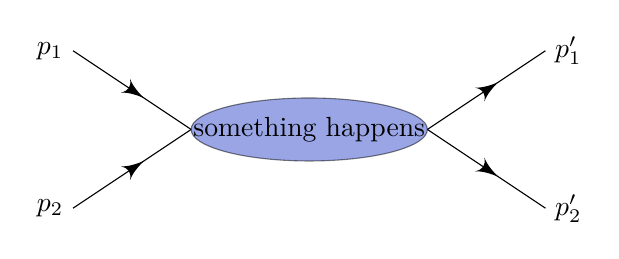
\begin{tikzpicture}
      \draw [->-=0.6] (-1.5, 1) node [left] {$p_1$} -- (0, 0);
      \draw [->-=0.6] (-1.5, -1) node [left] {$p_2$} -- (0, 0);
      \draw [fill=mblue, opacity=0.5] (1.5, 0) ellipse (1.5 and 0.4);
      \node at (1.5, 0) {something happens};
      \draw [->-=0.6] (3, 0) -- (4.5, 1) node [right] {$p_1'$};
      \draw [->-=0.6] (3, 0) -- (4.5, -1) node [right] {$p_2'$};
    \end{tikzpicture}
  \end{center}
  Then we have initial and final states
  \begin{align*}
    \bket{i} &= \sqrt{4 E_{\mathbf{p}_1} E_{\mathbf{p}_2}} b_{\mathbf{p}_1}^\dagger b_{\mathbf{p}_2}^\dagger\bket{0}\\
    \bket{i} &= \sqrt{4 E_{\mathbf{p}_1'} E_{\mathbf{p}_2'}} b_{\mathbf{p}_1'}^\dagger b_{\mathbf{p}_2'}^\dagger\bket{0}
  \end{align*}
  We look at the order $g^2$ term in $\brak{f}(S - I)\bket{i}$. We remove that $I$ as we are not interested in the case with no scattering, and we look at order $g^2$ because there is no order $g$ term.

  The second order term is given by
  \[
    \frac{(-ig)^2}{2}\int \d^4 x_1 \d^4 x_2 T\left[\psi^+(x_1) \psi(x_1) \phi(x_1) \psi^+(x_2) \psi(x_2) \phi(x_2)\right].
  \]
  Using Wick's theorem, there is a term in the string which is
  \[
    :\psi^\dagger(x_1) \psi(x_1) \psi^\dagger(x_2) \psi(x_2): \contraction{}{\phi}{(x_1)}{\phi}\phi(x_1)\phi(x_2).
  \]
  This contributes to the scattering because the two $\psi$ fields annihilate the initial $\psi$'s, whereas the $\psi^\dagger$'s create the final $\psi$'s. We can compute
  \begin{align*}
    &\brak{p_1', p_2'} ;\psi^\dagger(x_1) \psi(x_1) \psi^\dagger(x_2) \psi(x_2):\bket{p_1, p_2}\\
    \intertext{After some dreadful expansion in terms of creation and annihilation operators, we find that this is equal to}
    ={}&\brak{p_1', p_2'}:\psi^\dagger(x_1) \psi^\dagger(x_2):\bket{0} \brak{0}:\psi(x_1) \psi(x_2):\bket{p_1, p_2}\\
    ={}& (e^{ip_1' \cdot x_1 + i p_2' \cdot x_2} + e^{i p_1' \cdot x_2} + e^{ip_1' \cdot x_2 + p_2' \cdot x_1})(e^{-ip_1 \cdot x_1 - i p_2 \cdot x_2} + e^{-i p_1 \cdot x_2} - e^{-ip_2 \cdot x_1})\\
    ={}& e^{ix_1 \cdot (p_1' - p_1) + i x_2 \cdot (p_2' - p_2)} + e^{ix_1(p_2' - p_1) + i x_1 (p_1' - p_1)}
  \end{align*}
  Plus what we obtain by swapping $x_1$ and $x_2$.

  Putting this into the integral, we get
  \[
    \frac{(-ig)^2}{2}\int \d^4 x_1 \d^4 x_2 (\text{things}) + \int \frac{\d^4 k}{(2\pi)^4} \frac{e^{ik\cdot(x_1 - x_2)}}{k^2 - m^2 + i \varepsilon}.
  \]
  The $x_1x_2$ integrals give us delta functions. So we get
  \begin{align*}
    &(-ig)^2 \int \frac{\d^4 k}{(2\pi)^4} \frac{i (2\pi)^8}{k^2 - m^2 + i \varepsilon} \\
    &\hphantom{(-ig)^2 \int}(\delta^4(p_1' - p_1 + k) \delta^4(p_2' - p_2 - k) + \delta^4(p_2' - p_1 + k) \delta^4(p_1' - p_2 - k))\\
    ={}& (-ig)^2 \left(\frac{i}{(p_1 - p_1')^2 - m^2} + \frac{i}{(p_1 - p_2')^2 - m^2} - m^2\right)\\
    &\hphantom{(-ig)^2 \frac{i}{(p_1 - p_1')^2 - m^2} + \frac{i}{(p_1 - p_2')^2 - m^2}}(2\pi)^4 \delta^4(p_1 + p_2 - p_1' - p_2').
  \end{align*}
  What we see again is a $\delta$-function that enforces momentum conservation.
\end{eg}
As we've seen, this is tedious. We will see that there is an equivalent and easier to do this using Feynman diagrams. We draw diagrams to represent the expansion of $\brak{f}S\bket{i}$, and learn to associate numbers (or integrals) to them.

\subsection{Feynman diagrams}
We first describe the \term{Feynman diagrams} in words, then look at some examples.

The terms in the expansion can be represented pictorially as
\begin{itemize}
  \item Draw an external line for all particles in the initial and final states.
  \item Assign a directed momentum $p$ to each line, ie. an arrow into or out of the diagram to each line.

    We add an arrow for each $\psi$-particle to denote its charge: we chosen an incoming (outgoing) arrow in the initial state in the initial state for $\psi$ ($\bar{\psi}$ resp), and the reverse for the final state.
  \item Join the lines together with vertices to denote interactions
    \begin{center}
      \begin{tikzpicture}
        \begin{feynman}
          \vertex (i) {$\psi$};
          \vertex [right=of i] (a);
          \vertex [above right=of a] (f1) {$\psi$};
          \vertex [below right=of a] (f2) {$\bar{\psi}$};

          \diagram* {
            (i) -- [scalar] (a),
            (f1) -- [fermion] (a) -- [fermion] (f2),
          };
        \end{feynman}
      \end{tikzpicture}
    \end{center}
    Here the left dashed line represents $\phi$, the bottom-right arrow denotes $\psi^\dagger$, and the top-right arrow denotes $\psi$. Here the arrows matching up show that charge is conserved.

    We can add arrows to denote the momentum:
    \begin{center}
      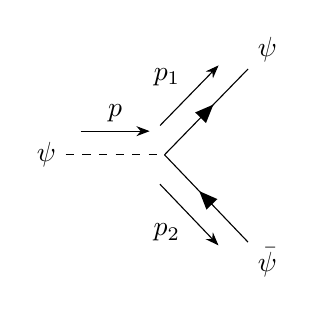
\begin{tikzpicture}
        \begin{feynman}
          \vertex (i) {$\psi$};
          \vertex [right=of i] (a);
          \vertex [above right=of a] (f1) {$\psi$};
          \vertex [below right=of a] (f2) {$\bar{\psi}$};

          \diagram* {
            (i) -- [scalar, momentum=$p$] (a),
            (f2) -- [fermion, reversed momentum=$p_2$] (a) -- [fermion, momentum=$p_1$] (f1),
          };
        \end{feynman}
      \end{tikzpicture}
    \end{center}
\end{itemize}
The allowed interactions are the terms present in the Lagrangian. For example, since we have a $\psi^\dagger\psi \phi$ term, we allow interactions that look like this:
\begin{center}
  \begin{tikzpicture}
    \begin{feynman}
      \vertex (i) {$\psi$};
      \vertex [right=of i] (a);
      \vertex [above right=of a] (f1) {$\psi$};
      \vertex [below right=of a] (f2) {$\bar{\psi}$};

      \diagram* {
        (i) -- [scalar] (a),
        (f1) -- [fermion] (a) -- [fermion] (f2),
      };
    \end{feynman}
  \end{tikzpicture}
\end{center}
The idea is that each such diagram is in one-to-one correspondence with a term in $\brak{f}(S - 1)\bket{i}$.

For example, if we look at $\psi + \psi \to \psi + \psi$, the simplest diagram is
\begin{center}
  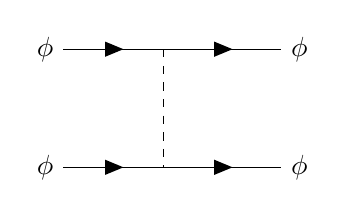
\begin{tikzpicture}
    \begin{feynman}
      \vertex (i1) {$\phi$};
      \vertex [below=of i1] (i2) {$\phi$};

      \vertex [right=of i1] (m1);
      \vertex [right=of m1] (f1) {$\phi$};
      \vertex [right=of i2] (m2);
      \vertex [right=of m2] (f2) {$\phi$};

      \diagram* {
        (i1) -- [fermion] (m1) -- [fermion] (f1),
        (i2) -- [fermion] (m2) -- [fermion] (f2),
        (m1) -- [scalar] (m2),
      };
    \end{feynman}
  \end{tikzpicture}
\end{center}
On the other hand, to enforce Bose statistics, we should also swap the directions:
\begin{center}
  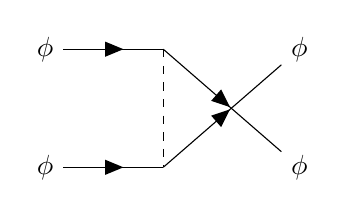
\begin{tikzpicture}
    \begin{feynman}
      \vertex (i1) {$\phi$};
      \vertex [below=of i1] (i2) {$\phi$};

      \vertex [right=of i1] (m1);
      \vertex [right=of m1] (f1) {$\phi$};
      \vertex [right=of i2] (m2);
      \vertex [right=of m2] (f2) {$\phi$};

      \diagram* {
        (i1) -- [fermion] (m1) -- [fermion] (f2),
        (i2) -- [fermion] (m2) -- [fermion] (f1),
        (m1) -- [scalar] (m2),
      };
    \end{feynman}
  \end{tikzpicture}
\end{center}
These are the ones that correspond to second-order terms. They are called the \term{Bom approximation}.

There are also more complicated ones such as
\begin{center}
  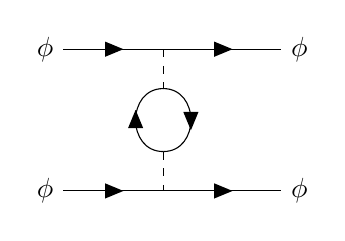
\begin{tikzpicture}
    \begin{feynman}
      \vertex (i1) {$\phi$};
      \vertex [below=1.8cm of i1] (i2) {$\phi$};

      \vertex [right=of i1] (m1);
      \vertex [right=of m1] (f1) {$\phi$};
      \vertex [right=of i2] (m2);
      \vertex [right=of m2] (f2) {$\phi$};

      \vertex [below=0.5cm of m1] (c1);
      \vertex [below=0.8cm of c1] (c2);

      \diagram* {
        (i1) -- [fermion] (m1) -- [fermion] (f1),
        (i2) -- [fermion] (m2) -- [fermion] (f2),
        (m1) -- [scalar] (c1) -- [fermion, half left] (c2) -- [fermion, half left] (c1),
        (c2) -- [scalar] (m2),
      };
    \end{feynman}
  \end{tikzpicture}
\end{center}
This is a \term{1-loop diagram}. We can also have a \term{2-loop diagram}:
\begin{center}
  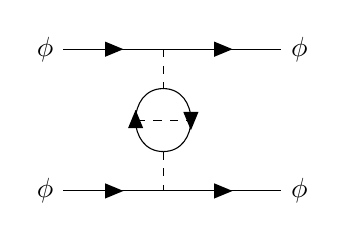
\begin{tikzpicture}
    \begin{feynman}
      \vertex (i1) {$\phi$};
      \vertex [below=1.8cm of i1] (i2) {$\phi$};

      \vertex [right=of i1] (m1);
      \vertex [right=of m1] (f1) {$\phi$};
      \vertex [right=of i2] (m2);
      \vertex [right=of m2] (f2) {$\phi$};

      \vertex [below=0.5cm of m1] (c1);
      \vertex [below=0.8cm of c1] (c2);

      \vertex [below right=0.4cm and 0.4cm of c1] (r);
      \vertex [below left=0.4cm and 0.4cm of c1] (l);
      \diagram* {
        (i1) -- [fermion] (m1) -- [fermion] (f1),
        (i2) -- [fermion] (m2) -- [fermion] (f2),
        (m1) -- [scalar] (c1) -- [fermion, half left] (c2) -- [fermion, half left] (c1),
        (c2) -- [scalar] (m2),
        (r) -- [scalar] (l),
      };
    \end{feynman}
  \end{tikzpicture}
\end{center}

If we ignore the loops, we say we are looking at the \term{tree level}.

To each such diagram, we associate a number using the \term{Feynman rules}.
\begin{enumerate}
  \item To each internal line $i$, we assign a momentum $k_i$.
  \item To each vertex $x$, we write a factor $(-ig)(2\pi)^4 \delta^4(\sum_i k_i)$, where the sum goes through all lines going into the vertex (and put a negative sign for those going out).
  \item For each internal line with momentum $k$, we have a factor
    \[
      \int \frac{\d^4 k}{(2\pi)^4} D(k^2),
    \]
    where
    \begin{align*}
      D(k^2) &= \frac{i}{k^2 - m^2 + i\varepsilon}\text{ for }\phi\\
      D(k^2) &= \frac{i}{k^2 - \mu^2 + i\varepsilon}\text{ for }\psi
    \end{align*}
\end{enumerate}

\begin{eg}
  We again look at
  We consider the case where $g$ is small. Then only the simple diagrams with very few vertices matter.
  \begin{center}
    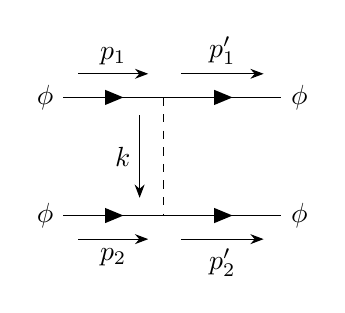
\begin{tikzpicture}
      \begin{feynman}
        \vertex (i1) {$\phi$};
        \vertex [below=of i1] (i2) {$\phi$};

        \vertex [right=of i1] (m1);
        \vertex [right=of m1] (f1) {$\phi$};
        \vertex [right=of i2] (m2);
        \vertex [right=of m2] (f2) {$\phi$};

        \diagram* {
          (i1) -- [fermion, momentum=$p_1$] (m1) -- [fermion, momentum=$p_1'$] (f1),
          (i2) -- [fermion, momentum'=$p_2$] (m2) -- [fermion, momentum'=$p_2'$] (f2),
          (m1) -- [scalar, momentum'=$k$] (m2),
        };
      \end{feynman}
    \end{tikzpicture}
    \quad
    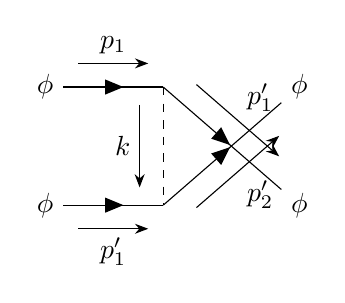
\begin{tikzpicture}
      \begin{feynman}
        \vertex (i1) {$\phi$};
        \vertex [below=of i1] (i2) {$\phi$};

        \vertex [right=of i1] (m1);
        \vertex [right=of m1] (f1) {$\phi$};
        \vertex [right=of i2] (m2);
        \vertex [right=of m2] (f2) {$\phi$};

        \diagram* {
          (i1) -- [fermion, momentum=$p_1$] (m1) -- [fermion, momentum=$p_1'$] (f2),
          (i2) -- [fermion, momentum'=$p_1'$] (m2) -- [fermion, momentum'=$p_2'$] (f1),
          (m1) -- [scalar, momentum'=$k$] (m2),
        };
      \end{feynman}
    \end{tikzpicture}
  \end{center}
  As promised by the Feynman rules, the two diagrams give us
  \[
    (-ig)^2 (2\pi)^8(\delta^4(p_1 - p_1' - k) \delta^4(p_2 + k - p_2') + \delta^4(p_1 - p_2' - k)\delta^4(p_2 + k - p_1').
  \]
  Now integrating gives us the formula
  \begin{multline*}
    (-ig)^2 \int \frac{\d^4 k}{(2\pi)^4} \frac{(2\pi)^8 i}{k^2 - m^2 + i \varepsilon} (\delta^4(p_1 - p_1' - k) \delta^4(p_2 + k - p_2') \\
    + \delta^4(p_1 - p_2' - k)\delta^4(p_2 + k - p_1')).
  \end{multline*}
  Doing the integral gives us the desired result.
\end{eg}
There is a nice physical interpretation of the diagrams. We can interpret the first diagram as saying that the nucleons exchange a meson of momentum $k = p_1 - p_1' = p_2 - p_2'$. This meson doesn't necessarily satisfy the relation $k^2 = m^2$. When this happens, we say it is \term{off-shell}, or that it is a \term{virtual meson}. Heuristically, it can't live long enough for its energy to be measured accurately. In contrast, the external legs are \term{on-shell}, so they satisfy $p_i^2 = m^2$.

\subsection{Amplitudes}
It is easy to perform the integral in the $\psi + \psi \to \psi + \psi$ at order $g^2$. We define the \term{amplitude} $\mathcal{A}_{f,i}$ as what we get by stripping off all the $4$-momentum conserving $\delta$-functions (this $\delta$-function follows from translational invariance, and is common to all $S$-matrix elements). So we have
\[
  \brak{f}S - I\bket{i} = i \mathcal{A}_{f,i}a (2\pi)^4 \delta^4 (p_F - p_I),
\]
where $p_F$ is the sum of final state $4$-momenta, and $F_I$ is the sum of initial state $4$-momenta. The factor of $i$ sticking out is by convention, to match with non-relativistic quantum mechanics.

We can now define our Feynman rules to compute $\mathcal{A}_{f, i}$.

\begin{itemize}
  \item Draw all possible diagrams with the appropriate external legs and impose $4$-momentum conservation at each vertex.
  \item Write a factor $(-ig)$ for each vertex.
  \item For each internal line, factor in the propagator.
  \item Integrate over $4$-momentum $k$ flowing in each loop.
\end{itemize}

\begin{eg}[Nucleon-antinucleon scattering]
  Consider another tree-level process
  \[
    \psi + \bar{\psi} \to \phi + \phi.
  \]
  We have a diagram of the form
  \begin{center}
    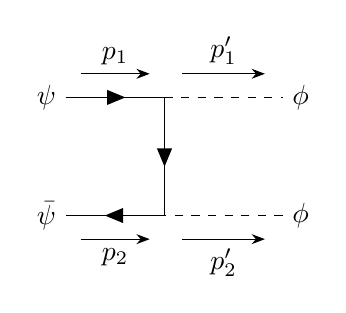
\begin{tikzpicture}
      \begin{feynman}
        \vertex (i1) {$\psi$};
        \vertex [below=of i1] (i2) {$\bar{\psi}$};

        \vertex [right=of i1] (m1);
        \vertex [right=of m1] (f1) {$\phi$};
        \vertex [right=of i2] (m2);
        \vertex [right=of m2] (f2) {$\phi$};

        \diagram* {
          (i1) -- [fermion, momentum=$p_1$] (m1) -- [scalar, momentum=$p_1'$] (f1),
          (f2) -- [scalar, rmomentum=$p_2'$] (m2) -- [fermion, rmomentum=$p_2$] (i2),
          (m1) -- [fermion] (m2),
        };
      \end{feynman}
    \end{tikzpicture}
  \end{center}
  and a similar one with the two $\phi$ particles crossing.

  The two diagrams then say
  \[
    \mathcal{A} = (-ig)^2 \left(\frac{1}{(p_1 - p_1')^2 - \mu^2} + \frac{1}{(p_2 - p_2')^2 - \mu^2}\right).
  \]
  Note that we dropped the $i\varepsilon$ terms in the denominator because the denominator never vanishes.
\end{eg}

\begin{eg}[Meson scattering]
  Consider
  \[
    \phi + \phi \to \phi + \phi.
  \]
  This is a bit more tricky. There is no tree-level diagram we can draw. The best we can get is a box diagram like this:
  \begin{center}
    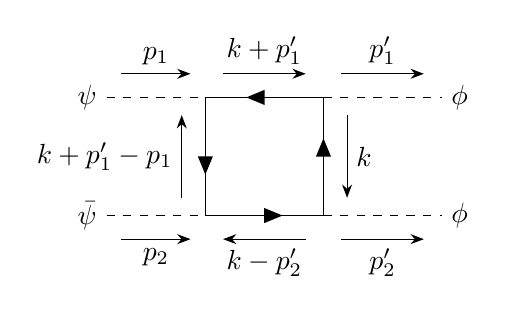
\begin{tikzpicture}
      \begin{feynman}
        \vertex (i1) {$\psi$};
        \vertex [below=of i1] (i2) {$\bar{\psi}$};

        \vertex [right=of i1] (m1);
        \vertex [right=of m1] (n1);
        \vertex [right=of n1] (f1) {$\phi$};
        \vertex [right=of i2] (m2);
        \vertex [right=of m2] (n2);
        \vertex [right=of n2] (f2) {$\phi$};

        \diagram* {
          (i1) -- [scalar, momentum=$p_1$] (m1),
          (i2) -- [scalar, momentum'=$p_2$] (m2),
          (n1) -- [scalar, momentum=$p_1'$] (f1),
          (n2) -- [scalar, momentum'=$p_2'$] (f2),

          (n1) -- [anti fermion, momentum=$k$] (n2) -- [anti fermion, momentum=$k - p_2'$] (m2) -- [anti fermion, momentum=$k + p_1' - p_1$] (m1) -- [anti fermion, momentum=$k + p_1'$] (n1);
        };
      \end{feynman}
    \end{tikzpicture}
  \end{center}
  We then integrate through all possible $k$.

  This particular graph we've written down gives
  \begin{multline*}
    i\mathcal{A} = (-ig)^4 \int \frac{\d^4 k}{(2\pi)^4}\\\frac{i^4}{(k^2 - \mu^2 + i\varepsilon)((k + p_1')^2 + \mu^2 + i\varepsilon)((k + p_1' - p_1)^2 - \mu^2 + i \varepsilon)((k - p_2)^2 - \mu^2 + i \varepsilon)}.
  \end{multline*}
  For large $k$, this asymptotically tends to $\int \frac{\d^4 k}{k^8}$, which fortunately converges. However, this is usually not the case. For example, we might have $\frac{\d^4k}{k^4}$, which diverges, or even $\int \frac{\d^4 k}{k^2}$. This is when we need to do renormalization.
\end{eg}
\printindex
\end{document}
